%% THIS IS THE MAIN FILE %%
% Here the main arrangement of your thesis is determined. 
% In this file you read-in all chapters (as separate .tex files)
% This is also the file you 'Build' with a LaTeX editor, like TeXmaker.
% The .cls file (MScThesis.cls) contains all details regarding copyrights and so on. Take a look and adjust where applicable. But be careful changing this file: it determines the whole lay-out of your thesis!
% This MSc thesis standard layout is optimized for double sided printing on A4 format paper.
% Good luck and have fun with your Master Research in Applied Geophysics! Kind regards, Niels Grobbe

\documentclass[a4paper,11pt]{MScThesis}
%
%\usepackage{pifont}
\mscName{Fabian Antonio Stamm}
\mscDate{\today}
\mscTitle{Test}
\mscSubTitle{Subtitle}
\mscKeyWords{thesis, msc, subject}
%
%\mscBackPicture{2660PF3}    % eps of 21 * 29.7 cm
\mscReaderOne{Prof. Florian Wellmann, Ph.D.}
\mscReaderTwo{Prof. Dr. Janos Urai}
\mscReaderThree{Miguel de la Varga, M.Sc.}
%\mscReaderFour{}
%
\setThesisInfo
%
\begin{document}
%
%============================= Front matter ========================================
\frontmatter %
%
% Make a hell of a lot of title pages
    \maketitle
%
% Abstract
    \nonumchap{Abstract}

Please pay particular attention to the preparation of your abstract; use this text as a guide. Every master thesis report must be accompanied by an informative abstract of no more than one paragraph (max 300 words). The abstract should be self-contained. No references, figures, tables, or equations are allowed in an abstract. Do not use new terminology in an abstract unless it is defined or is well-known from the literature. The abstract must not simply list the topics covered in the paper but should (1) state the scope and principal objectives of the research, (2) describe the methods used, (3) summarize the results, and (4) state the principal conclusions. Do not refer to the master thesis report itself in the abstract. For example, do not say, "In this thesis we will discuss". Furthermore the abstract must stand alone as a very short version of the master thesis report rather than as a description of the contents. Remember that the abstract will be the first and most widely read portion of the master thesis report. Readers will be influenced by the abstract to the point that they decide to read the master thesis report or not.

    \cleardoublepage
%
% Acknowledgements
    \nonumchap{Acknowledgements}%
    First of all I want to thank all the people who have participated in this project ..
    Remember, often more people have (in some way) contributed to your final thesis than you would initially think of....
    \vspace*{15mm}

    \noindent 
    RWTH Aachen University \hfill \mscname\\ % choose the university where you carried out your final MSc thesis research
    \mscdate

%
% table of contents, (\toc or \toclof or \tocloflot )
    \tocloflot
%
% Nomenclature
    \printnomencl %
%
% Acronyms
    \nonumchap{Acronyms} %
    %
    \begin{acronym}%
        \acro{RWTH}{Aachen University}%
    \end{acronym}%
    %
    \cleardoublepage%
%
%
%============================= Main matter =========================================
%
\mainmatter
%
% Introduction
\chapter{Introduction} \label{chap:intro}
Bayesian methods are an intuitive approach to inference, naturally inherent in human thinking patterns and closely tied to processes of decision-making \citep{berger2013stat, davidson2015, jaynes1986bayesian}. Individuals are constantly faced with situations in which a decision has to be made, but only incomplete information is available. Such a problem necessitates an approach based on plausible reasoning, one which is intuitively structured in five stages \citep{jaynes1986bayesian}:
\begin{enumerate}
	\item Identify uncertainties and attempt to consider all possibilities that might arise.
	\item Based on all the information and past experience available, evaluate how likely every possibility is.
	\item Assess the probable consequences of single possible actions.
	\item Based on the foregone steps, make a decision \citep{jaynes1986bayesian}.
\end{enumerate}
This concept is relatable to a vast variety of problems, ranging from casual every-day situations to complex scenarios in large-scale economic decision-making: As a private person, should I take an umbrella with me today? As a company, should we invest in the development and realization of a certain project? Following this process of plausible reasoning, the quality of a decision is to be measured based on the preceding state of knowledge and reasonable expectations, not on the subsequent actual consequences \citep{jaynes1986bayesian}. In other words: A decision is optimal, as long as it is the best action given the information available to the decision-maker before making the decision, no matter if actual loss was incurred afterwards.\\
Bayesian decision theory and the related concepts of expected loss and loss functions have found increasingly common application in several economic sectors and fields of research, such as medicine \citep{ashby2000evidence, ashby2006bayesian, moye2006statistical} and machine learning \citep{barber2012bayesian, theodoridis2015machine}. Probabilistic approaches to decision-making have also become prevalent in the sector of hydrocarbon exploration and production (SOURCE). However, the methods here a mainly limited on (p10-p90, decision trees).......(see BRATVOLD)???\\
In geosciences, Bayesian inference has prominently found use in the context of geophysical inversion problems (see \citet{tarantola1982inverse, mosegaard2002probabilistic} and \citet{sambridge2002monte}). Recently, it was transferred by \citet{delaVarga2016} to the field of structural geological modeling. This has been enabled by progressing developments regarding implicit geological modeling functions based on interpolation \citep{hillier2014three, mallet1992discrete, lajaunie1997foliation} and the possibility of fully automated model reconstruction in particular.  \citet{delaVarga2016} regarded geological modeling as a Bayesian inference problem by relating additional geological information to prior model parameters in the form of likelihood functions, linking them in a non-parametric Bayesian network. Using Markov chain Monte Carlo sampling to explore resulting probability spaces, they attained posterior model suites with reduced uncertainties \citep{delaVarga2016}\\
This work builds upon their concept, exploring the potential significance their findings might have in the context of decision-making. Bayesian decision-theory is to be included in the step of model evaluation. This is achieved by assigning an economic meaning to the structural model and designing a case-specific custom loss functions to find decisions which are optimal related to the state of knowledge and the preferences of actor's with different risk-affinities. More specifically, the models are designed to represent potential petroleum systems. Consequently, the development of algorithms for automatic hydrocarbon trap recognition and volume calculation represent a central part of this work.\\
The main hypothesis of this work is that Bayesian inference and resulting changes in uncertainties in a geological setting have a significant effect on related value estimation and decision-making. It is furthermore postulated that loss functions can be customized to appropriately represent preferences of actors in the hydrocarbon sector and moreover illustrate the nature of decisions such actor's might make depending on their individual attitudes towards risk and in the face of different types of uncertainties. Changes in their respective decisions are treated as a suitable measure to assess the effect of updating model parameters with new geological information. % notice how the reference to the introduction takes place.. It refers to the name.tex

\cleardoublepage

%
% First Part
    \part{First Part} % you can divide your thesis into different parts, for example Theory&Modeling in part 1 and real data examples in part 2.
		    \chapter{Methods}\label{cha:met}
    In the following chapter, we present the methodology utilized in this work. Bayesian analysis and decision theory are introduced in Section \ref{sec:bayes}. Focus is laid on Bayesian inference, estimation of uncertain values and the use of loss functions in this context. 
    We apply these methods in the context of structural geological modeling. Respective approaches to computational modeling, specifically in a probabilistic framework, are described in Section \ref{sec:bayes_in_struc_modeling}. Regarding numerical implementation, GemPy and PyMC are presented as central tools used in a Python environment. In Section \ref{sec:model_evaluation}, we outline our methods to evaluate consequent modeling results are. Particularly the potential for valuation from an economic perspective is elaborated in this regard and basic principles of subsurface hydrocarbon systems are introduced. Considering the respective setting in the economic sector of petroleum production, the development of an according case-specific custom loss function is described in Section \ref{sec:LF_design}. We first apply these methodologies on a conceptual 1D geological model (see Section \ref{sec:1D_model}), subsequently on a full 3D structural geological model. Design, construction and methods to identify hydrocarbon trap features in such the 3D model are explained in Section \ref{sec:3D_model}.
        
        \section{Bayesian analysis and decision theory}\label{sec:bayes}
	    As implied by the name, the problems and reasoning behind decision making are examined in the field of decision theory \citep{berger2013stat}. Such decision problems are commonly influenced by parameters that are uncertain. In statistical decision theory, available statistical knowledge is used to gain information on the nature of these uncertainties. Such uncertain parameters can be considered as numerical quantities. In order to find the best decision to a problem, it is possible to combine sample information with other aspects such as the possible consequences of decision making and the availability of prior information on our uncertainties. Decision consequences are expressed as gains in economic decision theory and as losses, which equal negative gains, in statistics. Prior information might be given for example based on experience from previous similar problems or from expert knowledge \citep{bratvold2010making}. The approach of utilizing priors is known as Bayesian analysis, which is explained in the following \citep{berger2013stat}. %(It goes well with decision theory.)
	    
	    \subsection{Basic elements}
	    First, some basic elements are to be defined. The unknown (uncertain) quantity influencing decision making is usually denominated as the state of nature $\theta$ \citep{berger2013stat}. Given statistical information on $\theta$ in the form of probability distributions, $\theta$ is called the parameter. 
	    Decisions are also referred to as actions $a$.
	    The outcome of statistical tests in form of information or statistical evidence is denoted as $y$.	    
	    Loss is defined as $L(\theta,a)$, so $L(\theta_1,a_1)$ is the actual loss incurred when action $a_1$ is taken while the true state of nature is $\theta_1$ \citep{berger2013stat}. Loss, expected loss and loss functions are explained in detail further below.  
        
        \subsection{Bayesian inference}
        Bayesian inference is most importantly characterized by its preservation of uncertainty, in contrast to standard statistical inference \citep{jaynes2003probability, box2011bayesian, harney2013bayesian, davidson2015}. The Bayesian approach is widely seen as intuitive and inherent in the natural human perspective. Probability is seen as a measure of belief for an event to occur. These beliefs can be assigned to individuals. Thus, different and even contradicting beliefs about the probability of an event might be held by different individuals, based on variations and disparities in the information available to each one individual.\\
        The initial belief or guess about an event $\theta$ can be denoted as $p(\theta)$. This is used as the so-called prior probability on which Bayesian updating is based. The beliefs about the occurrence of an event are revalued in the presence of additional information, i.e. the observation of new evidence $y$. These observations are included as likelihoods $p(y|\theta)$. By conducting this process of inference, a posterior probability $p(\theta|y)$ is attained. It is important to note that the prior is not simply discarded but re-weighted by Bayesian inference. By utilizing an uncertain prior, the potential for wrongfulness of the initial guess is already included. This means that Bayesian updating is about reducing uncertainty in a belief and reaching a guess that is less wrong. Bayesian inference is defined by and conducted via the following equation, called the Bayes' Theorem \citep{jaynes2003probability, box2011bayesian, harney2013bayesian, davidson2015}:
        \begin{equation}\label{eq:BayesTheorem}
        p(\theta|y) = \frac{p(y|\theta)p(\theta)}{p(y)}
        \propto p(y|\theta)p(\theta).
        \end{equation}
                
        \subsection{Estimation}
        The resulting posterior distribution can be used to acquire point estimates for the true state of nature $\theta$. Common and simple examples for such estimators are the mode (i.e. the generalized maximum likelihood estimate), the mean and the median of a distribution \citep{berger2013stat}. The presentation of a point estimate should usually come with a measure for its estimation error. According to \citet{berger2013stat}, the posterior variance is most commonly used as an indication for estimate accuracy. However, it is argued by \citet{davidson2015} that by using pure accuracy metrics, while this technique is objective, it ignores the original intention of conducting the statistical inference in cases, in which payoffs of decisions are valued more than their accuracies. A more appropriate approach can be seen in the introduction of loss and the use of loss functions \citep{davidson2015}.
        
        \subsection{Expected loss and loss functions}\label{sec:loss} 
        Loss is a statistical measure of how "bad" an estimate is, i.e. how much is lost by making a certain decision. Gains are considered by statisticians as negative losses.
        The magnitude of incurred loss related to an estimate is defined by a loss function, which is a function of the estimate of the parameter and the true value of the parameter \citep{wald1950statistical, davidson2015}:        
        \begin{equation}\label{eq:LossFunction}
        L(\theta,\hat{\theta}) = f(\theta,\hat{\theta}).
        \end{equation}        
        So, how "bad" a current estimate is, depends on the way a loss function weighs accuracy errors and returns respective losses. Two standard loss functions are the absolute-error and the squared-error loss function. Both are simple to understand and commonly used \citep{davidson2015}.\\        
        As implied by its name, the absolute-error loss function returns loss as the absolute error, i.e. the difference between the estimate and the true parameter \citep{davidson2015}:        
        \begin{equation}\label{eq:AbsLossFunction}
        L(\theta,\hat{\theta}) = |\theta - \hat{\theta}|.
        \end{equation}                
        Accordingly, losses increasing linearly with the distance to the true value are returned for respective estimates. This means that all differences between relative errors are weighed equally, no matter whether they are found in the realm of relatively small or relatively large errors \citep{hennig2007}.\\
        Using the squared-error loss function returns losses that increase quadratically with distance of the estimator to the true parameter value \citep{davidson2015, moye2006statistical}:        
        \begin{equation}\label{eq:SqrLossFunction}
        L(\theta,\hat{\theta}) = |\theta - \hat{\theta}|^2.
        \end{equation}         
        This exponential growth of loss also means that large errors are weighed much stronger than small errors. This might come with over-valuation of distant outliers and misrepresentation of magnitudes in distance. Regarding this, the absolute-error loss function can be seen as more robust \citep{davidson2015}.
        \begin{figure}[h]
        	\centering
        	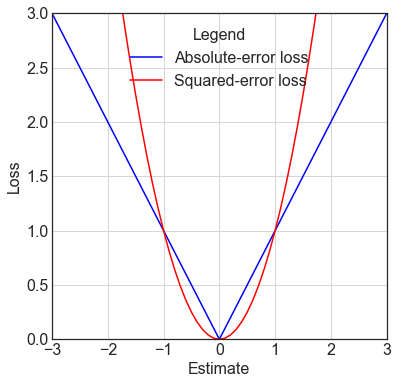
\includegraphics[width=0.5\textwidth]{Figures/abs_sqr_det.png}
        	\caption{Realizations of loss based on the absolute-error loss function (blue) and the squared-error loss function (red) for a determined true value $\theta$ = 0.}\label{fig:abs_sqr_det} 
        \end{figure}\\
        Both of these standard loss functions are symmetric and can be described as objectively aiming at a high precision in estimating the true parameter value (see Figure \ref{fig:abs_sqr_det}).
        \citet{davidson2015} and \citet{hennig2007} propose that it might be useful to move away from these type of objective loss functions to the design of customized loss functions that specifically reflect an individual's (i.e. the decision maker's) objectives, preferences and outcomes. \citet{hennig2007} argue that choosing and designing a loss function involves the translation of informal aims and interests into mathematical terms. This process naturally implies the integration of subjective decisions and subjective elements. According to \citet{hennig2007}, this is not necessarily unfavorable or "less objective", as it may better reflect an expert's perspective on the situation and contribute to a productive scientific discussion.\\        
        The standard loss functions defined above are symmetric, but can easily be adapted to be asymmetric, for example by weighing errors on the negative side stronger than those on the positive side. Preference over estimates larger than the true value (i.e. overestimation) is thus incorporated in an uncomplicated way \citep{davidson2015, hennig2007}. Much more complicated designs of loss functions are possible, depending on purpose, objective and application \citep{davidson2015}. A case-specific loss functions is designed in Section \ref{sec:LF_design} of this work.\\
        The presence of uncertainty during decision making implies that the true parameter is unknown and thus the truly incurred loss $L(\theta,a)$ cannot be known at the time of making the decision \citep{berger2013stat, davidson2015}. The Bayesian perspective considers unknown parameters as random variables and samples that are drawn from the posterior distribution as possible realizations of the unknown parameter, i.e. all possible true values are represented by this distribution \citep{davidson2015}. A probabilistic alternative to the actual loss is to consider each decision's expected loss and to make a decision that is optimal in relation to this expected loss \citep{berger2013stat}. \\        
        Given a posterior distribution $p(\theta|y)$, the expected loss of choosing an estimate $\hat{\theta}$ over the true parameter $\theta$ (after evidence $y$ has been observed) is defined by the function below \citep{davidson2015}:
        
        \begin{equation}\label{eq:ExpectedLoss}
        l(\hat{\theta}) = E_{\theta}[L(\theta,\hat{\theta})].
        \end{equation}  
        
        \begin{figure}[h]
        	\centering
        	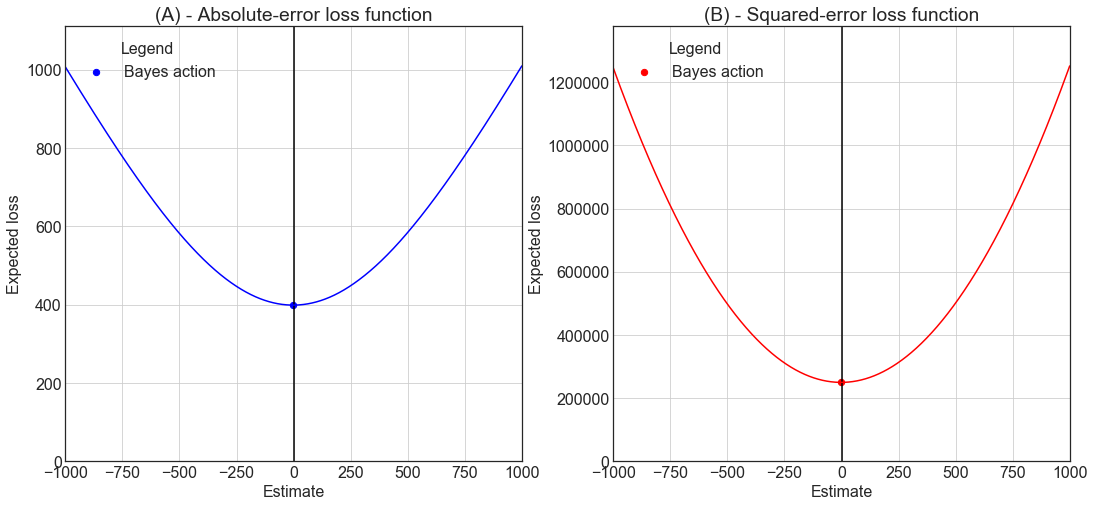
\includegraphics[width=1\textwidth]{Figures/loss_functions.png}
        	\caption{Expected loss and respective Bayes actions based on the standard absolute-error loss (A) and squared-loss function (B). In this example, we applied the functions on a normal distribution characterized by $\mu = 0$ and $\sigma = 500$.}\label{fig:standard_LF} 
        \end{figure}
        
        The expectation symbol $E$ is subscripted with $\theta$, by which it is indicated that $\theta$ is the respective unknown variable. This expected loss $l$ is also referred to as the Bayes risk of estimate $\hat{\theta}$ \citep{berger2013stat, davidson2015}. Exemplary realizations of the expected loss according to both standard loss functions and minimized by the Bayes action are plotted in Figure \ref{fig:standard_LF}.\\        
        By the Law of Large Numbers, the expected loss of $\hat{\theta}$ can be approximated drawing a large sample size $N$ from the posterior distribution, respectively applying a loss function $L$ and averaging over the number of samples \citep{davidson2015}:
        
        \begin{equation}\label{eq:ExpectedLoss2}
        \frac{1}{N}\sum_{i=1}^{N} L(\theta_i,\hat{\theta}) \approx E_{\theta}[L(\theta,\hat{\theta})] = l(\hat{\theta}).
        \end{equation}
        
        Minimization of a loss function returns a Bayesian point estimate known as Bayes action or Bayesian estimator $\delta^p(y)$, which is the estimate, action or decision with the least expected loss according to the loss function \citep{berger2013stat, moye2006statistical}. For a unimodal and symmetric absolute-error loss function, the Bayes action is simply the median of the posterior distribution, while using squared-error loss it is the mean \citep{davidson2015, berger2013stat}. The MAP (maximum a posteriori) estimate is the minimizing solution for the posterior using zero-one loss \citep{davidson2015}. The possibility of more than one minimum also implies that several Bayes actions can exist for one problem \citep{berger2013stat}.\\
        \citet{davidson2015} implemented different risk affinities by simply  introducing a risk parameter into the loss function. By using different values for this parameter, it can be represented how comfortable an individual is with being wrong and furthermore which "side of wrong" is preferred by this decision maker \citep{davidson2015}. This approach to expressing risk-affinities is used for the design of the custom loss functions in Section \ref{sec:LF_design}.
        
        %\subsection{Value of information}
        %- considering the change in gain (or loss) after regarding new information or evidence, the value of this information can be calculated
        %- in the presence of uncertainty we look at expected value of information
        %- this can be used as a measure, to assess if the effort to attain new evidence or information is worth it
        %- also as a measure to see how much additional information is worth to different actors with different risk affinities
        %- here we use the comparison between Bayes actions before and after Bayesian updating
        
        \section{Application in structural geological modeling}\label{sec:bayes_in_struc_modeling}
        In this work, these methods of Bayesian analysis and decision theory are applied in the field of geological structural modeling. The fundamental approach follows closely the research conducted by \citet{delaVarga2016} and builds upon their findings.\\
        According to them, structural geological modeling can be regarded as a statistical problem and the elements of Bayesian inference can be specified in this context as follows:
        \begin{enumerate}
        	\item \textbf{Mathematical forward model ($M$)}: The connections between parameters $\theta$ and observed data $y$ are defined in such mathematical models. According to \citet{wellmann2010towards} and \citet{delaVarga2016}, the realization of a geological model $M$ can be regarded as a direct function of a set of input parameters:
        	\begin{equation}
        	M = f(\vec{x}, \phi_i, k_j, \alpha_k, \beta_l)\label{eq:forward_model},
        	\end{equation}
        	where $\phi_i$ is a function of position $\vec{x}$, more precisely an interpolation function, to which respective additional interpolation parameters are given by $\alpha_k$. Available primary geological information, such as positions and dips of layer interfaces, is represented by $k_j$. A topological description, such as the relationships between faults and layer surfaces, is given by $\beta_\ell$. An essential aspect of this function is that it allows for a full automation of the modeling step, so that the consequences of a change in an input parameter are realized directly without the need for any further manual inspection or interaction \citep{wellmann2017sandstone, delaVarga2016}. The modeling step and the respective interpolation method used in this work are presented in Section \ref{sec:struc_geo_modeling} below.
        	\item \textbf{Model parameters ($\theta$)}: These model-defining parameters can be deterministic or stochastic. In the latter case, they are uncertain parameters to which a probability distribution is assigned. Regarding Equation \ref{eq:forward_model} above, these can be any of the factors $\vec{x}$, $k_j$, $\alpha_k$ and $\beta_l$, which define the realization of the forward model over $\phi_i$.
        	\item \textbf{Observed data ($y$)}: This is any type of additional information that can be related to the forward modeling results or to the parameters and their combinations, and might possibly be used to reduce uncertainty. Such data can be gained by measurements and observations, for example by core sampling, well-log analysis or seismic acquisition. 
        	\item \textbf{Likelihood functions $p(y|\theta)$}: Links between the previous parameters $\theta$ and the additional data $y$ are established by these functions in a way that they reflect the likelihood of the parameter states given the observations. They are mathematically defined in the same way as probability functions, but are a function of the data $y$, instead of the parameters $\theta$ \citep{mackay2003information, patil2010pymc, delaVarga2016}.
        \end{enumerate}
        
        A fundamental sequence of the inference process was proposed by \citet{gelman2014bayesian}, adapted by \citet{delaVarga2016} and is subsequently adjusted for the application in this work as follows:
        \begin{enumerate}
        	\item \textbf{Setting up a full probability model}: A multi-dimensional joint probability space is to be generated, taking into account the probability distributions of every model parameter $\theta$. A 2D example is illustrated in Figure \ref{fig:joint_prob}.
	        \begin{figure}[h]
				\centering
				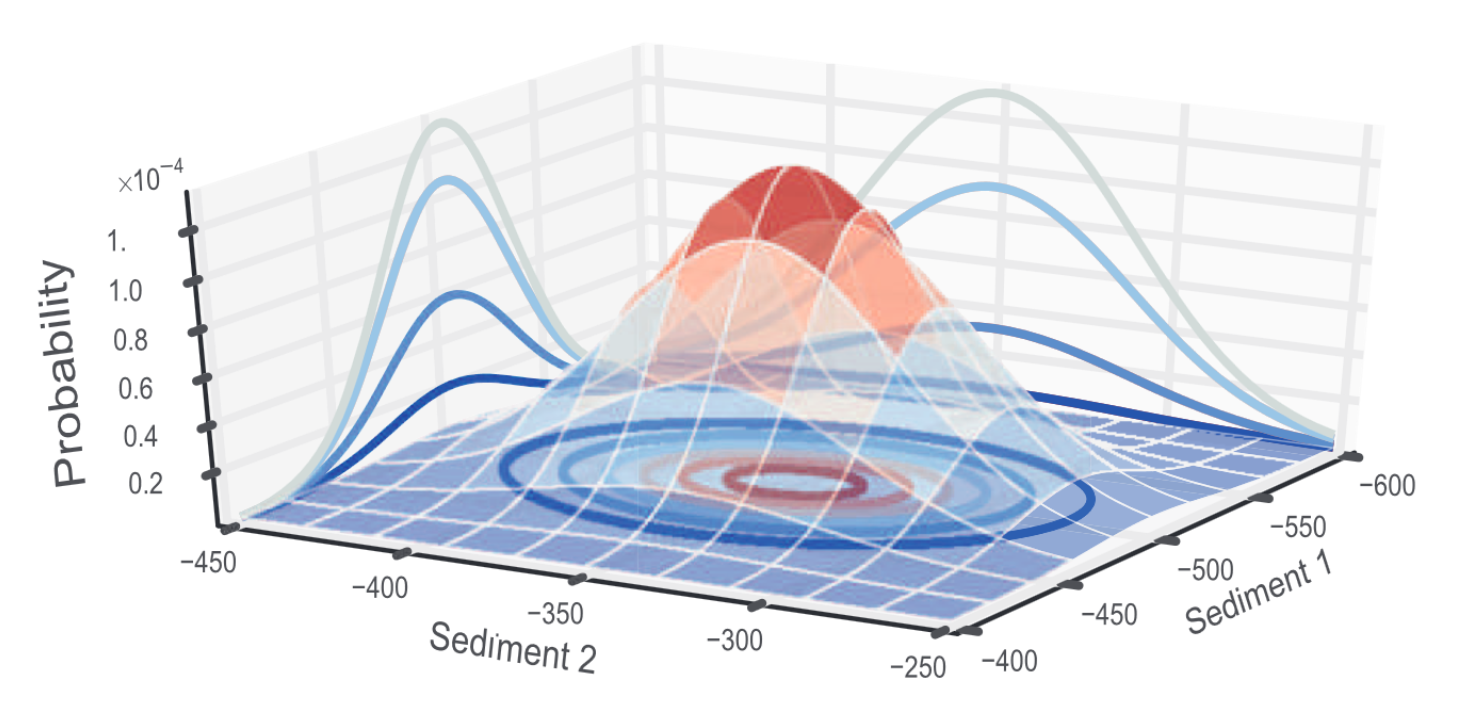
\includegraphics[width=0.8\textwidth]{Figures/joint_prob}
				\caption{Example visualization of a 2D joint probability space generated by two random parameters $\theta$ (from \citet{delaVarga2016}).}\label{fig:joint_prob} 
			\end{figure}
        	\item \textbf{Conditioning on observed data}: Subsequently, an appropriate posterior distribution $p(\theta|y)$ is to be calculated by conditioning the parameters $\theta$ on the observed data $y$ given the likelihood $p(y|\theta)$. This is the step of Bayesian updating of the belief about the parameter uncertainty given new information.
        	In a chosen model ($M$), this is achieved by linking parameters and data through deterministic operations to the likelihood functions. It is pointed out by \citet{delaVarga2016} that any combination of parameter-observation connections is allowed, i.e. not all parameters need to be necessarily connected to all observed data. After all conditional probabilities have been set up, the Bayes Theorem (Equation \ref{eq:BayesTheorem}) is applied to attain the posterior \citep{delaVarga2016}. However, due to the multi-dimensionality given in geological problems, the use of Markov chain Monte Carlo methods is advised to achieve this as described in Section \ref{sec:mcmc} below.
        	\item \textbf{Evaluation of the posterior model}: Depending on the aim of the study, a post-processing analysis can be conducted accordingly. \citet{delaVarga2016} focused on the examination of the posterior distributions of the parameters $\theta$ and the generated models, particularly regarding information entropy within the model space. In this work, the geological models are additionally assigned an economic meaning by declaring them potential petroleum reservoirs and introducing customized loss functions to reflect the economic interest of decision makers in developing respective resource extraction projects (see Section \ref{sec:loss}). Changes in Bayes actions are considered a measure for the influence of Bayesian inference on decision making and the significance of additional observations for different decision makers.
        \end{enumerate}
        
        \subsection{Markov chain Monte Carlo sampling (MCMC)}\label{sec:mcmc}
        Despite the apparent simplicity of the Bayes Theorem, a direct analytical calculation and exact inference of the posterior distribution $p(\theta|y)$ is rarely possible in non-idealized cases, due to intractability in multi-dimensional spaces \citep{hoffman2014no, delaVarga2016}. Thereby arises the necessity to resort to methods of statistical inference approximation. Markov chain Monte Carlo (MCMC) sampling has proven to be a generally applicable and reliable method for exploring multi-dimensional parameter spaces in an intelligent way \citep{hoffman2014no, davidson2015}. \citet{gilks2005markov} has emphasized the significance of MCMC for the application in Bayesian statistics in particular.\\
        %In Monte Carlo integration, random samples are drawn from a target distribution, such as our posterior distribution P(A$|$X), to approximate the integral or probability density function in terms of an expectation:
        %\begin{equation}\label{eq:MonteCarlo}
        %        E[P(A|X)] \approx \frac{1}{N}\sum_{n=1}^{N}P(A|X)
        %\end{equation}
        In the ordinary Monte Carlo approach, random independent samples are drawn from a target distribution in order to approximate its shape \citep{gilks2005markov, delaVarga2016}. High-dimensional parameter spaces as found in Bayesian applications lead to vast spaces of likelihood and often make independent sampling infeasible \citep{gilks2005markov}. This can be solved by extending the Monte Carlo principle with a Markov chain, in which every sample iteration of the parameter $\theta^{(t+1)}$ is dependent uniquely on the previous value $\theta^{(t)}$ \citep{gilks2005markov, delaVarga2016}.\\
        The general principle of MCMC can be described as follows: 
        Drawing representative samples from a target distribution of unknown shape is based on the conduction of a so-called random walk on the parameter distribution space. $T$ sampling steps are to be performed. The first sampling location is chosen at random. With each subsequent step, a new position is proposed. The new sample value is then related to the previous step. According to a weight defined by the scaled-up candidate density of the value, the proposed step is then accepted or rejected. In the case of acceptance, the value is added to the sample trace and the process is continued from the current location. In the case of rejection, sampling is reverted to the previous accepted step \citep{schaaf2017, delaVarga2016}. After performing the complete number of $T$ iterations, all accepted sampling locations (i.e. the trace) are returned. The intention behind this concept it to achieve convergence of the sampling algorithm towards areas of high probability \citep{davidson2015}.\\ 
        Variations in the way of how new  sample steps are proposed and in the acceptance-rejection condition result in different single MCMC sampling methods \citep{schaaf2017, delaVarga2016}. Various algorithms for random MCMC walks have been developed for over more than six decades and advancements have still been made in recent years. Common examples for such algorithms are the Metropolis-Hastings samplers as devised by \citet{metropolis1953equation} and generalized by \citet{hastings1970}. The Gibbs sampler \citep{geman1984stochastic} is another well-known method. 
        For the purpose of this work, an adaptive Metropolis-Hastings sampler is used.\\
        In Metropolis-Hastings methods, each sampling step at iteration $t$ is determined by a candidate probability distribution $q(\theta,\theta^{'})$, from which a proposed sample $\theta^{'}$ is drawn. The acceptance-rejection condition is defined by the acceptance ratio $a(\theta^{'},\theta)$ \citep{haario2001adaptive}:
        
        \begin{equation}\label{eq:acceptance_ratio}
        a(\theta^{'},\theta)=\frac{p(\theta^{'})p(y|\theta^{'})}{p(\theta)p(y|\theta)}.
        \end{equation}
        
        To ensure a thorough exploration of the probability space, the transition to higher probability densities should not be enforced in every case but selectively. This is assured by relating the acceptance ratio from Equation \ref{eq:acceptance_ratio} to a random value $u$ from a Uniform distribution $U(0,1)$ as follows \citep{delaVarga2016}:
        
        \begin{equation}\label{eq:transition_selectivity}
        \theta^{(t+1)}=\begin{cases}
        \theta^{'} & $if $ a(\theta^{'},\theta)>U(0,1)\\
        \theta^{t} & $otherwise$\\
        \end{cases}.
        \end{equation}
        
        Thereby, the algorithm assigns high probabilities to high-density points and low probabilities to low-density points, so that the chain state is moved accordingly \citep{delaVarga2016}.\\
        Metropolis methods are furthermore defined by the step size scale factor that is chosen. While large steps are good for exploration of the space and mixture in the chain, acceptance rates are low. Small steps have better acceptance rates, but lead to slower exploration and convergence of the algorithm \citep{delaVarga2016}.\\
        For the iterative sampling in this work, Adaptive Metropolis (AM) by \citet{haario2001adaptive} is used. It adapts the traditional Metropolis-Hastings by incorporating the ability of continuous step-size tuning during convergence, by taking into account the full information saved along the process. This is achieved by generating a covariance matrix that is updated every iteration. The adaptive nature of the process enables fast convergence for non-linear distributions while maintaining ergodicity \citep{haario2001adaptive, delaVarga2016}. Its suitability for multi-dimensional distribution spaces make it an excellent method for dealing with complex models such as structural geological models \citep{schaaf2017}.\\
        For sampling, a large enough number of iterations $T$ has to be chosen, so that a reliable and statistically significant exploration of the parameter space is assured. This is primarily dependent on the rate of convergence towards the true distribution. Considering empirical Bayes methods, in which either priors or likelihoods stem from empirical data, as is assumed for the models in this work, convergence can be expected to be reached almost immediately \citep{delaVarga2016}. However, for high dimensional problems more iterations are required, in order to ensure an accurate representation of posterior distributions \citep{wellmann2017sandstone}. Different realizations of the full 3D geological model are then constructed on the basis of the approximated posterior distributions, using an implicit modeling step described in the following.
        
        \subsection{Structural geological forward modeling}\label{sec:struc_geo_modeling}       
        Performing forward modeling in the context of structural geology requires the use of a suitable modeling step $M$ (see Equation \ref{eq:forward_model}). For the application in a probabilistic setting, the method should enable fully automatic reconstruction of the model, when parameters are changed. The application in this work follows the example of \citet{wellmann2010towards} and \citet{delaVarga2016}, and relies on the use of implicit interpolation for geological modeling, a method developed and elaborated by \citet{lajaunie1997foliation} and \citet{calcagno2008geological}.\\
        This implicit method relies on the interpolation of a potential field scalar function $T(\vec{x})$ of any point $\vec{x}$ in a 3D space, and thus reflects the geometry of geological structures \citep{calcagno2008geological}. Modeling $T(\vec{x})$ is achieved by cokriging two forms of data: (i) contact points on geological interfaces through increments of the potential field $T(\vec{x})-T(\vec{x}^{\,'})$ and (ii) orientation data as gradients, i.e. partial derivatives of the potential field $\delta T(\vec{x})/\delta u_\beta$ in each directon $u$ \citep{calcagno2008geological}. The respective estimator is defined as follows:
        \begin{equation}\label{eq:Cokriging_Estimator}
                T(\vec{x})-T(\vec{x_0})=\sum_{\alpha=1}^{M}\mu_\alpha(T\vec{x_\alpha}-T(\vec{x}^{\,'}_\alpha))+\sum_{\beta=1}^{N}\nu_\beta\frac{\delta T}{\delta u_\beta}(\vec{x}_\beta),
        \end{equation}        
        where $\vec{x_0}$ is an arbitrary origin, $M$ and $N$ are the total number of data points and partial derivatives respectively, and their relative contributions are weighed by the factors $\mu_\alpha$ and $\nu_\beta$. Furthermore, $T$ is assumed to be a random function defined by polynomial drift and a stationary covariance $K(h)$ \citep{calcagno2008geological}. The use of a cubic covariance model is suggested by \citet{calcagno2008geological}, based on the results from studies conducted by \citet{aug2004modelisation} and \citet{chiles2004modelling}.
		\begin{figure}[h]
			\centering
			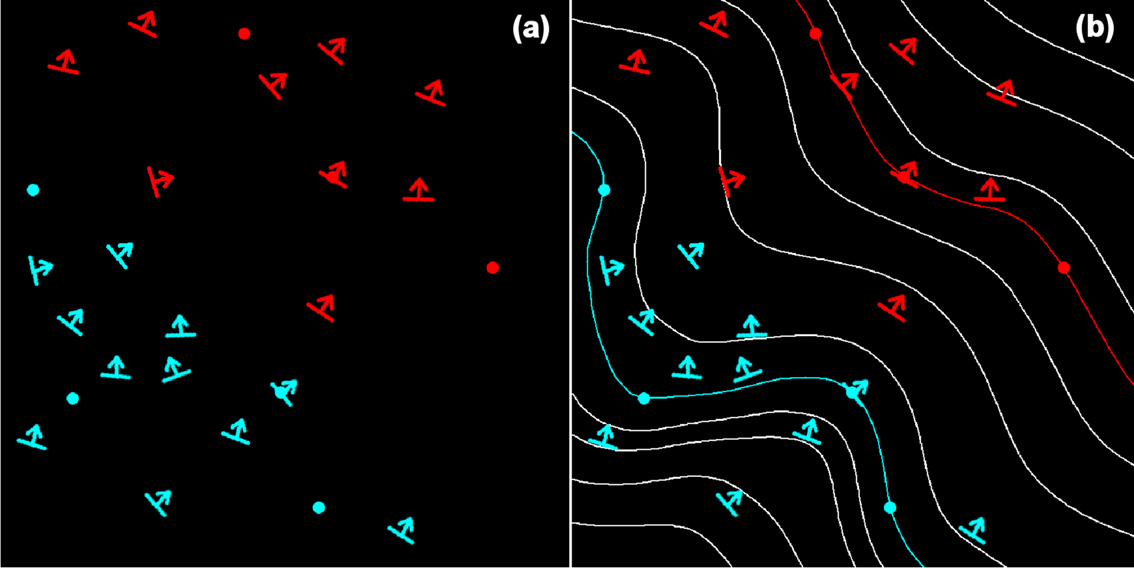
\includegraphics[width=1\textwidth]{Figures/calcagno_pot_field.png}
			\caption{Illustration of the concept of interpolating to attain a poentail field. The original data is depicted in (a), with contact points as dots and orientation measurements indicated by arrows. Colors represent respective assignments to different formations. An accordingly calculated potential field is shown in (b) (from \citet{calcagno2008geological}).}\label{fig:pot_field}
		\end{figure}        
        Resulting potential fields can be used to describe geological interfaces as iso-surfaces in any kind of 3D geometry \citep{calcagno2008geological}. Fault geometries can be interpolated analogously. These can be infinite in the 3D space, interrelated in a fault network or finite. To account for the effect of faults on geological layers, discontinuous potential fields are created by applying discontinuous drift functions in the cokriging system. Additionally, geological rules allow for the representation of several types of interactions between sets of geological layers \citep{calcagno2008geological}.\\
        It is pointed out by \citet{calcagno2008geological}, that this method is particularly appropriate for cases in which knowledge about the geology is only given for sparse locations and is thus applicable for a wide variety of typical problems in geological settings. Its suitability for this work is furthermore emphasized by the possibility to modify the topology-defining geological pile to achieve different geometric realizations without altering the data. The model can thus be updated in the face of new data or interpretations \citep{calcagno2008geological}. 
     
		\subsection{Numerical computational implementation via Python, GemPy and PyMC}\label{sec:numerical_implementation}
		Bayesian analysis can be conducted numerically using probabilistic programming methods \citep{salvatier2016pymc3}. The implicit method of forward geological modeling, described above, is to be embedded in such a framework. For doing so, the programming language of choice in this work is Python. The merits of Python have been pointed out by \citet{behnel2010}, \citet{Langtangen2008} and \citet{salvatier2016pymc3}. Development is facilitated by an expressive but concise and clean syntax that is easy to learn. Python is dynamic, compatible with multiple platforms and offers good support for numerical computing. Integration of other scientific libraries and extension via C, C++, Fortran or Cython are easily possible \citep{behnel2010, salvatier2016pymc3, Langtangen2008}. Python is thus a straightforward tool for the implementation of central components of Bayesian analysis, such as custom statistical distributions and samplers \citep{salvatier2016pymc3}.\\
		The 3D geological modeling step in this work is implemented using GeMpy, an open-source, Python-based software that is able to generate and visualize complex 3D structural geological models based on the potential field interpolation method elaborated in Section \ref{sec:struc_geo_modeling} \citep{delaVarga2017gempy}. Its design allows for its application in a probabilistic setting as elaborated below. At the time of writing this, GemPy is still under development (version 0.995), but is already functioning for the purpose of this work.\\
		For conducting the Bayesian analysis and embedding the geological modeling step in a probabilistic context, GemPy is integrated into the probabilistic framework of PyMC. This Python library was developed for conducting Bayesian inference and prediction problems in an open-source probabilistic programming environment \citep{davidson2015, salvatier2016pymc3}. Different model fitting techniques are provided in PyMC, such as the \textit{maximum a posteriori} (MAP) method and several (MCMC) sampling methods, including the Adaptive Metropolis introduced in Section \ref{sec:mcmc}. The components which are used to construct a statistical model, are represented by \textit{Deterministic} or \textit{Stochastic} functions in PyMC \citep{salvatier2016pymc3}. These variables are described as hierarchically related nodes, specifically parent and child nodes, in a Bayesian network:
		\begin{enumerate}
			\item \textbf{Parent} nodes include variables that affect other variables.
			\item \textbf{Child} nodes contain variables that are influenced by other variables (they depend on parent variables) \citep{delaVarga2016}.
		\end{enumerate}
		The values of \textit{Deterministic} variables are completely dependent on its parents' values, as defined by a respective mathematical function \citep{salvatier2016pymc3}. \textit{Stochastic} variables are used to represent uncertain parameters $\theta$ or observed stochastic variables as likelihood functions $p(y|\theta)$ \citep{salvatier2016pymc3, delaVarga2016}. Complex mathematical relations between \textit{Stochastic} variables can be described through \textit{Deterministic} functions \citep{delaVarga2016}. Futhermore, PyMC allows for the creation of own object definitions inheriting from the class descriptions of these two variable types.\\
		Bayesian networks as a concept have been presented in more detail by \citet{koller2009probabilistic}. \citet{salvatier2016pymc3} have pointed out that the development of PyMC is continuing, as the inclusion of further tools is planned for future updates.
		%While conducting MCMC sampling, a burn-function can be implemented via PyMC, through which it can be defined that the $t_b$ first trace samples are discarded. This can be useful to d\\		
		
		
		%\subsection{Bayesian hierarchical networks}\label{sec:hierarchical_bayes}
		\section{Model evaluation}\label{sec:model_evaluation}
        After conducting Bayesian inference, posterior distributions and resulting model realizations are to be evaluated. For this, the sampling traces and posterior distributions of single parameters can be observed. The entirety of accepted 3D geological models (sampled after burn-in phase) is to be assessed in terms of uncertainty quantification. Furthermore, a central part of this work is the assignment of an economic significance to the modeling results. To achieve this, realized models are evaluated by regarding them as potential hydrocarbon systems. This process is further in Section \ref{sec:Reservoir_values}. Information entropy is introduced as a measure for uncertainty in the following.
        
        \subsection{Visualizing uncertainty}
        \begin{figure}
	        \centering
	        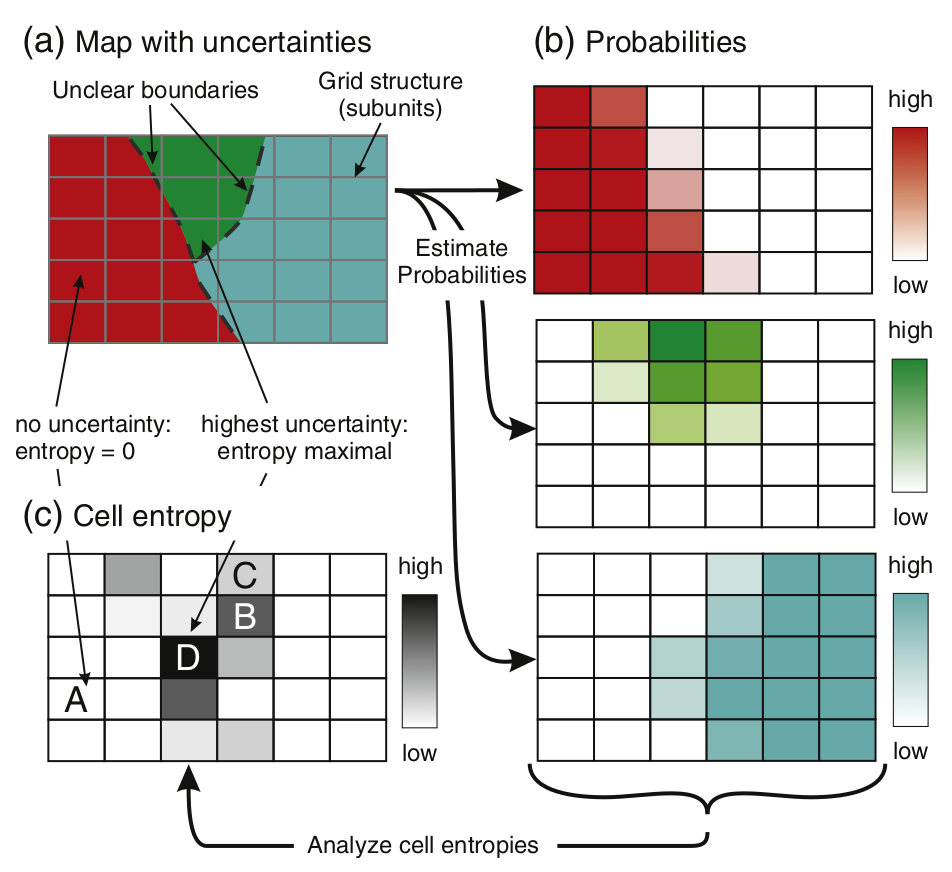
\includegraphics[width=1\textwidth]{Figures/information_entropy.png}
	        \caption{Illustrations depicting the concept of Shannon entropy to visualize uncertainties in spatial applications. In (a), a map composed of uncertain units is subdivided into a regular grid of equally sized cells. The probabilities of possible outcomes regarding each unit is estimated for each cell in (b). From this results a map of cell Shannon entropies (c), with the highest values where all units can occur equally frequent, and lowest for cells where no uncertainty is given and entropy is zero (from \citet{wellmann2012uncertainties}).}\label{fig:information_entropy}
        \end{figure}
        Shannon entropy, commonly also referred to as information entropy, was first defined by \citet{shannon1948mathematical} and adopted as a method to visualize uncertainties in 3D geological models by \citet{wellmann2012uncertainties}. This approach was later also used by \citet{delaVarga2016} and \citet{schaaf2017}. Shannon entropy is applied to predict the model accuracy at every location in the model space by visualizing its respective uncertainty and thus returning a measure for the quality of the model. This is achieved by subdiving the model space into a regular raster of equally sized cells (voxels) and measuring the accuracy for every such cell. In the context of geological modeling, the central question is based on the knowledge of how frequent a single geological feature occurs in a voxel \citep{wellmann2012uncertainties}. \citet{de1972definition} established that Shannon entropy can serve as a measure of fuzziness, a concept described by \citet{zadeh1965fuzzy}. Given a fuzzy set in which fuzziness of each part is indicated by $f\in [0,1]$, the following conditions hold:
        \begin{enumerate}
	        \item The measure should only be 0 if $f$ is 0 or 1 in every cell.
	        \item The measure is maximal given $f = 0.5$ in every cell \citep{de1972definition}.
        \end{enumerate}
        While the first condition represents the complete absence of uncertainty everywhere in the model, the second condition is met in the opposite case of full uncertainty in the whole model space, i.e. all outcomes are equally likely in each cell \citep{schaaf2017}. From this, the following equation for application in geological modeling was derived \citet{Mann1993,wellmann2012uncertainties}:
        \begin{equation}
	        H_m = -\frac{1}{N}*\sum_{x=1}^{N}[p_m(x)*\log(p_m(x))+(1-p_m(x))*\log(1-p_m(x))],
        \end{equation}
        in which $f$ is denoted as the probability $p_m$ of an outcome $m\in M$ in a cell with a position $x$. The fuzziness is quantified as the entropy $H_m$, normalized by the total number of cells $N$. Subsequently, an average Shannon entropy can be calculated for a model as \citep{wellmann2012uncertainties}:
        \begin{equation}
	        H_T = -\frac{1}{N}\sum_{x=1}^{N}H(x).
        \end{equation}
        This total entropy $H_T$ is 0 when no uncertainty is found in any cell, oppositely it is maximal in the case of equal probabilities of outcomes in every cell \citep{wellmann2012uncertainties, schaaf2017}. The application of these entropy measures allows for the calculation and visualization of uncertainties in each voxel, the assessment of uncertainties of entire geological units, as well as the quantification of total model uncertainty represented by a single number \citep{wellmann2012uncertainties}.
        
        \subsection{Economic significance of structural geological models as hydrocarbon systems}\label{sec:Reservoir_values}
        In this work, the generated structural geological models are to be assigned an economic significance in order to approach a real setting, in which hypothetical actors could have an interest in taking a decision, and thus, to evaluate the influence of the Bayesian inference of the decision making process. Changes in Bayes actions are considered as a measure for this effect. For this purpose, it is assumed that a hydrocarbon reservoir system is represented by each geological model realization.
        Such hydrocarbon systems are typically comprised of:
        \begin{enumerate}
        	\item \textbf{Source rock:} A kerogen-rich source rock which produced and emitted hydrocarbons during its burial history, given sufficient heating, is needed to provide oil or gas in the first place \citep{dolson2016basics}. These are typically organic-rich sedimentary rocks, shales in particular. For the purpose of this work, it is assumed that a  suitable source rock is present and hydrocarbons expulsion took place after the formation of any trap-defining structures in our geological models.
        	\item \textbf{Migration pathway:} A pathway that allows expelled oil and gas to migrate upwards through the subsurface from the source rock into potential reservoir formations is necessary \citep{dolson2016basics}. This condition is also assumed to be given in our model. Basement formations in the geological model are simply defined to be permeable.
        	\item \textbf{Seal}: These are formations that are able to halt hydrocarbons on their migration pathway as top, lateral and possibly bottom seals \citep{dolson2016basics, sorkhabi2005place}. Such sealing is generally defined by a reduction of pore space geometry relative to migration energy. Sealing is thus defined primarily by changes in stratigraphical composition to low porosities and micro-sized pore throats. These are characterized by a high capillary entry pressure able to resist the buoyancy pressure of hydrocarbons. This capillary pressure is also the main controlling factor for seal capacity. Lithologically, seals are most commonly comprised of shales, siltstones, tight carbonates, evaporites and salts \citep{dolson2016basics, dolson2016quantifying, sorkhabi2005place}. An additional factor to sealing is posed by the presence of faults. Fault zones may possess significantly higher or lower permeabilities then surrounding rock formations, which means that they may serve as fluid flow conduits or migration barriers respectively \citep{van2003lateral, sorkhabi2005place}. The possible influence of faults on structural hydrocarbon traps is elaborated in further detail below. For the model in this work, the cap rock is assumed to be a shale.
        	\item \textbf{Reservoir formations:} Suitable lithologies, in which hydrocarbon volumes can be stored, have to be present. For this, a suitable percentage of void space, i.e. a sufficiently high porosity, is required in a rock formation. Further significant factors are the connectivity of the porosity through pore throats, as well as pore geometry and resulting permeability \citep{dolson2016basics, sorkhabi2005place}. The larger the pore throats, the easier it is for fluids to migrate in a rock. Typical reservoir rocks are sandstones and carbonates, but even normally tight lithologies might serve as reservoirs, if they are fractured \citep{dolson2016basics}. In the models of this work, reservoir formations are assumed to be conventional sandstones.
        	\item \textbf{Trap:} Entrapment results from an appropriate reservoir-seal sequence and a three-dimensional geometric closure. Regarding a top view on a structural relief, closure is generally defined by any intersection of a structural contour and the seal, that is closed on both sides \citep{dolson2016basics, sorkhabi2005place}. A point at which a contour fails to close is referred to as "spill point". The maximum column depth to which a trap can be filled, and ultimately its maximum volume, is defined by this spill point. A trap that contains hydrocarbons down to the spill point is thus referred to as "filled to spill". Traps can also be "filled to seal capacity" when the seal capacity is exceeded by the buoyant pressure of a fill column of greater height. Lower accumulations can also result from insufficient migration, i.e. low charge volumes of oil or gas in the first place. Such a trap is referred to as "charge limited" \citep{dolson2016basics}. Many different types of traps, in which hydrocarbons can accumulate, are possible. A common trap type is a structural four-way closure, i.e. as reservoir-seal system that was folded into closed anticlines, often resembling a dome and is thus predominantly defined by the structural closure relief and the cap rock sealing capacity. Such a trap type can be considered to be closed, as the reservoir surface contours are closed in a circle or oval around a relief high. Closure can also be given through the intersection of a fault with the seal \citep{dolson2016basics}. Two common examples for traps are illustrated in Figure \ref{fig:trap_types}.
        \end{enumerate}
        \begin{figure}[h]
        	\centering
        	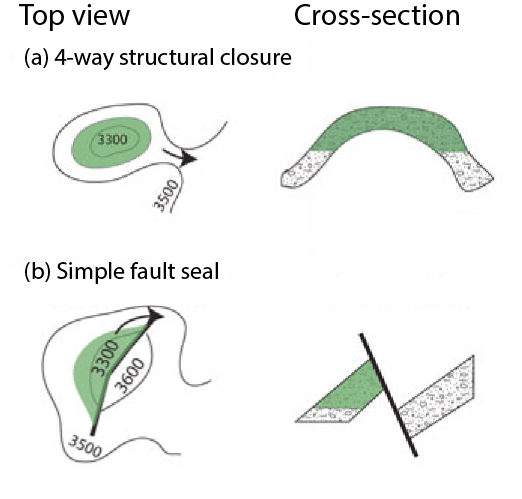
\includegraphics[width=0.5\textwidth]{Figures/trap_closure1}
        	\caption{Conceptual examples of a dome-shaped four-way-closure and a simple fault trap from top view (relief contour) and cross section perspective (modified from \citet{dolson2016basics}.}\label{fig:trap_types}
        \end{figure}        
        %The influence of faults and fault sealing potential on structural traps has been outlined by several researches such as \citet{sorkhabi2005place} and \citet{van2003lateral}.
        The presence of a fault in the reservoir-seal sequence can have different impacts on trap closure and the volume of a hydrocarbon accumulation. This is mainly defined by the transport properties of a fault, i.e. in which way it behaves as a seal or flow conduit respectively. Cases might range from complete fault sealing to complete leakage along a fault zone. More complex in-between cases are possible, such as faults that leak across, but are sealed along their plane. This ultimately defines the depth to which a trap may be filled and whether this point is controlled by a point of leakage on the fault plane or a spill point related to the remainder of the 3D structural closure. Another decisive aspects to consider, is the nature of juxtapositions across the fault, especially regarding the possibility of cross-fault leakage \citep{van2003lateral}. This is summarized in Figure \ref{fig:fault_trap_spills}.
		\begin{figure}[h]
			%\centering
			\begin{subfigure}{.8\textwidth}
				\centering
				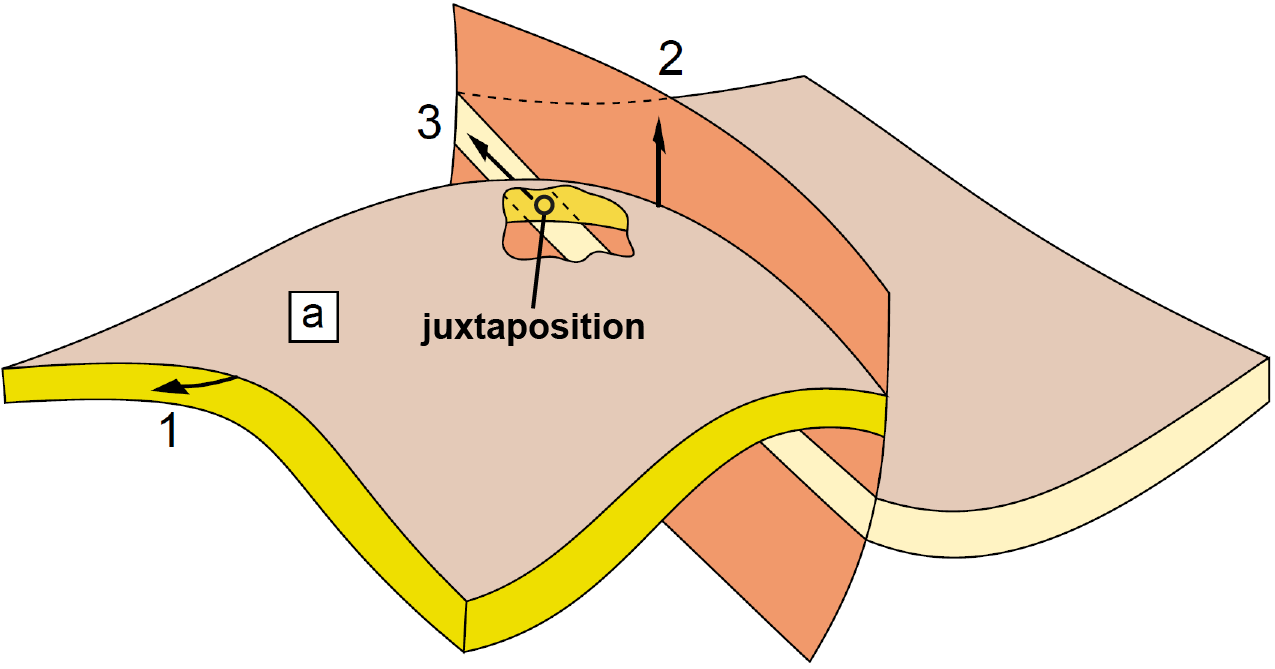
\includegraphics[width=1\linewidth]{Figures/fault_trap_mechA1}
				%\caption{Graph and saddle point of the function $z=x2~-~y2$.}\label{fig:saddle_point} 
			\end{subfigure}
			\begin{subfigure}{0.18\textwidth}
				\centering
				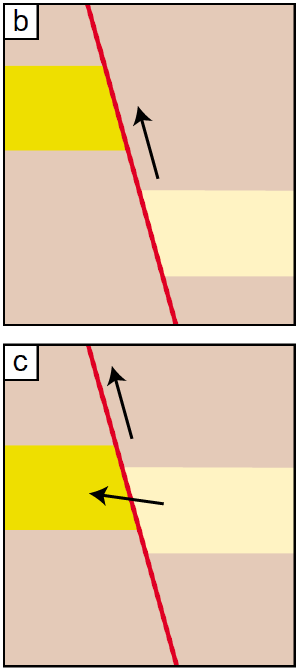
\includegraphics[width=1\linewidth]{Figures/fault_trap_mechB1}
				%\caption{Saddle point between two maxima.}\label{fig:saddle_point_between_maxima} 
			\end{subfigure}
			\caption{In (a), a structural trap resulting from the combination of 4-way anticlinal closure and a simple normal fault is illustrated. The two reservoir layers in both sides are juxtaposed, so that the hydrocarbon accumulation potential is controlled by three points of possible leak pathways: (1) the anticlinal spill point, (2) leakage upwards along the fault and (3) leakage across the fault enabled by the juxtaposition. Possibilities (2) and (3) depend on the transport properties of the fault zone, i.e. potential fault sealing. Given leakage along the fault (2), that size volume would be reduced to a small relatively small volume solely defined by the 4-way closure down to maximum contact of the reservoir-seal boundary with the fault plane. In case (b), the reservoirs are not juxtaposed and thus laterally sealed. Fault-related leakage can thus only occur along the plane. Leakage along and across the fault is enabled by the juxtaposition in (c) (modified from \citet{van2003lateral}).}\label{fig:fault_trap_spills}
		\end{figure}\\
		The transport properties of a fault zone are primarily defined by the internal structure and composition of its fault gouge. Fault gouge properties and ultimately the variation in permeability in the fault zone is primarily dependent on clay content. Clay smearing has thus been a central topic of research surrounding fault sealing (see \citet{lindsay1993outcrop, yielding1997quantitative, van2003lateral, van2005processes, schmatz2010clay}. It generally is defined as all processes that lead to the incorporation of clay from the wall rock (e.g. a shale as seal) into the fault zone \citep{van2003lateral, vrolijk2016clay}. Clay smearing can be described using different equations, such as the Shale Smear Factor ($SSF$) and the Shale Gouge Ratio ($SGR$) \citep{lindsay1993outcrop, yielding1997quantitative, vrolijk2016clay}. The $SSF$ provides a simple conceptual approach to assessing the clay smearing on a fault plane, dependent on ratio of fault throw magnitude $D$ to displaced shale thickness $T$ \citep{lindsay1993outcrop, yielding1997quantitative, yielding2012using} (see Figure \ref{fig:ssf}):
		\begin{equation}
			SSF = \frac{D}{T}.
		\end{equation}
		\begin{figure}[h]
			\centering
			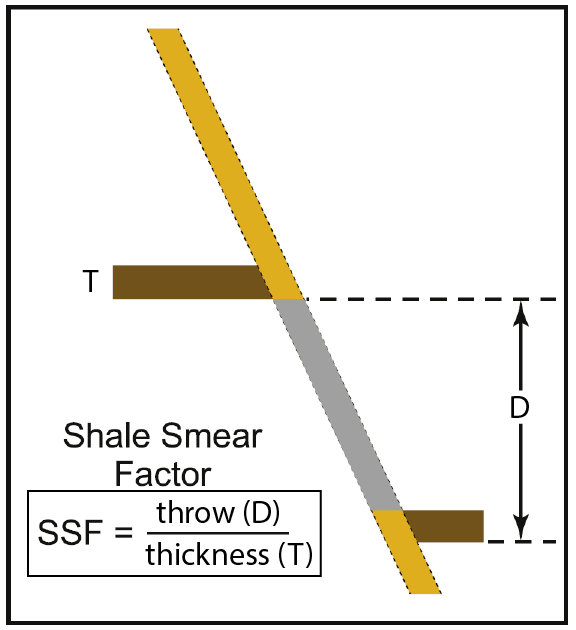
\includegraphics[width=0.7\textwidth]{Figures/SSF.PNG}
			\caption{Conceptual fault section illustrating the SSF approach to assess shale smear potential (modified from \citet{vrolijk2016clay}.)}\label{fig:ssf}
		\end{figure}
		It has been observed, that as the displacement and thus the ratio increases, a critical value $SSF_c$ will be reached, at which the clay smear is breached and no longer continuous. Initial observations by \citet{lindsay1993outcrop} indicated this threshold to be $SSF_c$ = 7. However, the critical value was later suggested to be scale-dependent and smaller for thick clays displaced by large faults \citep{yielding2012using}. \citet{faerseth2006shale} reported that for such large scales, including fault throws greater than 100~m, clay smear continuity can be expected for $SSF\le4$. Any larger values come with a decrease in confidence \citep{faerseth2006shale}. A critical review of the research on clay smearing published over the last four decades was recently presented by \citet{vrolijk2016clay}.			
        The 3D structural model in this work (see Section \ref{sec:3D_design}) is designed in a way that a potential conventional hydrocarbon trap is included in the form of anticlinal folding combined with normal faulting of a reservoir-seal sequence. Results from modeling are to be evaluated in a way that respective estimations on the basis of loss functions can be conducted, i.e. Bayesian decision theory is applicable. In the typical petroleum industrial setting, the main question is one of how much of the resource can be produced and how high the return on investment will be \citep{dean2007volumetric}. Thus, several of the factors named above are to be considered to attain a calculable volume of the structural trap which can further be economically interpreted using the approaches presented below.
        
        \subsection{Original oil-in-place and recoverable volumes as value measures}
        Before pressure and production tests have been conducted (i.e. before production has started), volumetric estimation is the only approach to assess the amount of hydrocarbons in place in a reservoir. From this value, recoverable reserves can be deduced based on an estimated recovery factor \citep{dean2007volumetric}.\\
        Oil-in-place and gas-in-place volumes are calculated based on:
        \begin{enumerate}
        \item Subsurface rock volume containing hydrocarbons. This is mainly defined by thickness and areal extend of the accumulation.
        \item Weighted average effective porosity of the reservoir rock.
        \item Water saturation in the reservoir rock.
        \item Hydrocarbon fluid properties \citep{dean2007volumetric}.
        \end{enumerate}
        As the hydrocarbon systems in this work are purely artificial, a pure oil accumulation is assumed for simplicity. Furthermore, defined formations are regarded as homogeneous in their lithological composition and petrological properties It is assumed, for example, that no shale is interbedded in the main sandstone reservoir unit. Using the factors listed above, the equation for original oil-in-place ($OOIP$) is formulated as follows:
        \begin{equation}\label{eq:OOIP}
        OOIP = A * h * \phi * (1 - S_W) * 1/FvF,
        \end{equation}
        where $OOIP$ is returned in $m^3$. The hydrocarbon-filled rock volume is defined by the drainage area $A$ in $m^2$ and the net pay thickness $h$ in $m$. Porosity $\phi$ and water saturation $S_W$ (interstitial water) are given in fractions of the rock volume. A dimensionless factor for the change in oil volume between reservoir conditions and standard conditions at surface is represented by the formation volume factor $FvF$. Thus, shrinkage of the oil volume brought to the surface is determined by $1/FvF$ \citep{dean2007volumetric}.\\
        Subsequently, the effectively recoverable oil volumes ($ROV$) can be calculated by multiplying the $OOIP$ with a recovery factor $RF$ \citep{dean2007volumetric}:
        \begin{equation}\label{eq:ROV}
                ROV = OOIP * RF = A * h * \phi * (1 - S_W) * 1/FvF * RF.
        \end{equation}
        The recovery factor is influenced by a number of fluid properties, such as viscosity, density, solution oil/gas ratio and the formation volume factor. Thus, it is difficult to estimate \citep{dean2007volumetric}. Globally, the ultimate average recovery factor for oil fields is about 35\% \citep{labastie2011increasingRF}. For gas accumulations, however, recovery factors range typically between 70 and 90\% \citep{dean2007volumetric}.\\
        In this work, the constructed geological models focus on the representation of the structural control in this equation. This refers in particular to potential structural traps and ultimately the hydrocarbon-filled rock volume represented by $A * h$ in Equations \ref{eq:OOIP} and \ref{eq:ROV}.
        Including the remaining factors as simple uncertain parameters would be easily possible and is usually done in the probabilistic estimation procedures commonly conducted in the petroleum industry \citep{wim2001guidelines}. However, the focus of this work lies on the structural aspects of a hydrocarbon system. Respective results and observations might possibly be overprinted and distorted by the incorporation of other parameters of petrology and engineering as uncertain. Effects of interest might become unrecognizable. Thus, fixed values are used for the non-structural factors ($\phi=30\%$, $S_W=20\%$, $FvF=1.05$, $RF = 80\%$). These are chosen arbitrarily but within a realistic range to considering a conventional oil reservoir. Consequently, calculating the $ROV$ from the maximum trap volume simply equates a rescaling of values, as proportions are conserved. However, translation of trap volumes to recoverable oil volumes is deemed appropriate for a formally better consideration of the results in the respective context of decision making in the hydrocarbon sector.\\
        %For most factors, it seems most suitable to define a normal distribution around a known typical value or global average, as it will return a high probability for common scenarios and occasionally produce cases of rare, more extreme values.\\ 
        Attaining the hydrocarbon-filled rock volume (i.e. the maximum trap volume) and calculating the $ROV$ is a central step of the model evaluation. Model realizations are hereby assigned the economic value on which decisions are to be based. Realized volumetric values from numerous iterations and several simulations are combined to sets of probability distributions of the $ROV$. Considering the $ROV$ as the true value to be estimated, loss functions can then be applied as described in Section \ref{sec:loss}. $OOIP$ and $ROV$ calculations are applicable in a 3D setting, the 1D geological model introduced below in Section \ref{sec:1D_model}, however, requires the use of an abstract valuation system.
        %\subsubsection{Net present value}
        %hmmm...
		
		\section{Designing a case-specific loss function}\label{sec:LF_design}	
		As explained before in Section \ref{sec:loss}, the standard symmetric loss functions provide objectively good estimators minimizing expected loss by returning the median or mean respectively. However, assigning an economic notion to our model and assuming the case of an actor or decision maker in any field, naturally necessitates the consideration of preferences, interests and the overall subjective perspective such an individual or for example a company might have. Further constraints, properties and factors can also be specific to the field, industry or generally to the problem at hand. Consequently, the design of a more specific non-standard and possibly asymmetric loss function might be required, so that an adapted Bayesian estimator can be found. One that includes subjective aspects and difference in weighting of particular gains or losses, arising from an actor's inherent preferences and the environment in which the actor has to estimate or make a decision. In the face of several uncertain parameters, a perfectly true estimate is virtually unattainable. However, an attempt can be made to design a customized loss function that returns a Bayesian estimator involving the least bad consequences for an individual in a specific environment. Assuming the reservoir setting case and valuation methods introduced in Section \ref{sec:Reservoir_values}), such a customization attempt is made and explained step by step in the following.\\
		%%%(SOURCES?)
		For the purpose of estimation, it makes sense that one of the standard loss functions is chosen as a basis and a customized loss function is developed from there. The absolute-error loss seems most appropriate for this case of hydrocarbon reservoir value estimation. Ideally, an actor would like to know the exact true value of interest, say the $OOIP$, so that investments or resources can be allocated appropriately in order to acquire economic gains. This allocation is the decision to be made or action to be taken. Deviations from the unknown true value in the form of over- and underestimation bring about an error and loss accordingly. In this case, it is assumed that investments increase linearly with linear growth in the value of the reserve. For this reason, the absolute-error loss function is favored here over the squared-error loss function. It is chosen as the base function to which further development steps refer, based on logical case-specific assumptions. The steps are illustrated in Figure \ref{fig:LF_4steps_normal} and listed in the following:
		\begin{figure}[p!]
			\centering
			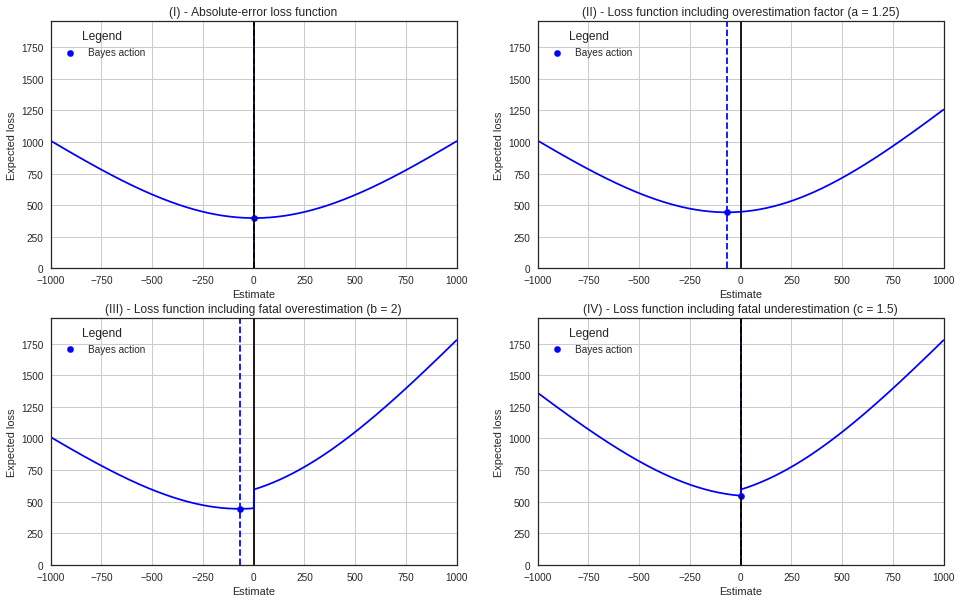
\includegraphics[width=1\textwidth]{Figures/LF_4steps_normal.png}
			\caption{Single steps (I-IV) of customizing the loss function applied on an exemplary normal distribution ($\mu=0; \sigma=500$). The median (in this case also mean and average) is returned for the Bayes action, when using the standard symmetric absolute-error loss function (I). Assigning a stronger weight on overestimation steepens the curve on the right hand side and shifts the minimum to the left, i.e. to a lower estimate (II). Steepening is significantly reinforced by the introduction of fatal overestimation in (III). This affects only the positive side of estimates and leads to a jump at zero, where signs change. Due to a similar condition, the same effect is observed on the negative side of estimate values, where the curve is also steepened, after including fatal underestimation (IV). Due to this, the Bayes action is shifted back to the zero estimate. The final custom loss function is represented by the curve in (IV).}\label{fig:LF_4steps_normal}
			\centering
		\end{figure}		
		\begin{enumerate}
			\item \textbf{Step I}: The standard symmetrical absolute-error loss function is chosen as a starting point for further customization steps:
			
			\begin{equation}
			L(\theta,\hat{\theta}) = |\theta - \hat{\theta}|.
			\end{equation}  
			
			\item \textbf{Step II}: Considering the development of a hydrocarbon reservoir, it can be assumed that over-investing is worse than under-investing. Overestimating the size of an accumulation might for example lead to the installation of equipment or facilites that are actually redundant or unnecessary. This would come with additional unrecoverable expenditures. Consequences from underestimating, however, may presumably be easier to resolve. Additional equipment can often be installed later on. Hence, overestimation is weighted stronger in this loss function by multiplying the error with an overestimation factor $a$:
			
			\begin{equation}\label{eq:LF_II}
			L(\theta,\hat{\theta}) = |(\theta-\hat{\theta})|*a.
			\end{equation}
			
			\item \textbf{Step III}: The worst case for any project would be that its development is set into motion, expecting a gain, only to discover later that the value in the reservoir does not cover the costs of realizing the project, resulting in an overall loss. A petroleum system might also turn out to be a complete failure, containing no value at all, although the actor's estimate indicated the opposite. Here, this is referred to as worst case or fatal overestimation. A positive value is estimated, but the true value is zero or negative. This is worse than the "normal" non-fatal overestimation, where both values are positive and a net gain is still achieved, which is only smaller then the best possible gain of expecting the true value. Fatal overestimation is included in the loss function by using another weighting factor $b$ that replaces \textit{a}:
			
			\begin{equation}\label{eq:LF_III}
			L(\theta,\hat{\theta}) = |(\theta-\hat{\theta})|*b.
			\end{equation}
			
			In other words: With $b = 2$, fatal overestimation is twice as bad as simple underestimation.
			
			\item \textbf{Step IV}: A worst case or fatal underestimation can also be derived from the idea of estimating a zero or negative value, when the true value is actually positive. This is assumed to be worse than non-fatal overestimation, but clearly better than fatal overestimation. No already owned resources are wasted, it is only the potential value that is lost, i.e. opportunity costs that arise from completely discarding a reservoir with a potential gain equal to the positive true value. Fatal underestimation is weighted using a third factor:
					
			\begin{equation}\label{eq:LF_IV}
			L(\theta,\hat{\theta}) = |(\theta-\hat{\theta})|*c.
			\end{equation}			
		\end{enumerate}
		\begin{figure}[h]
			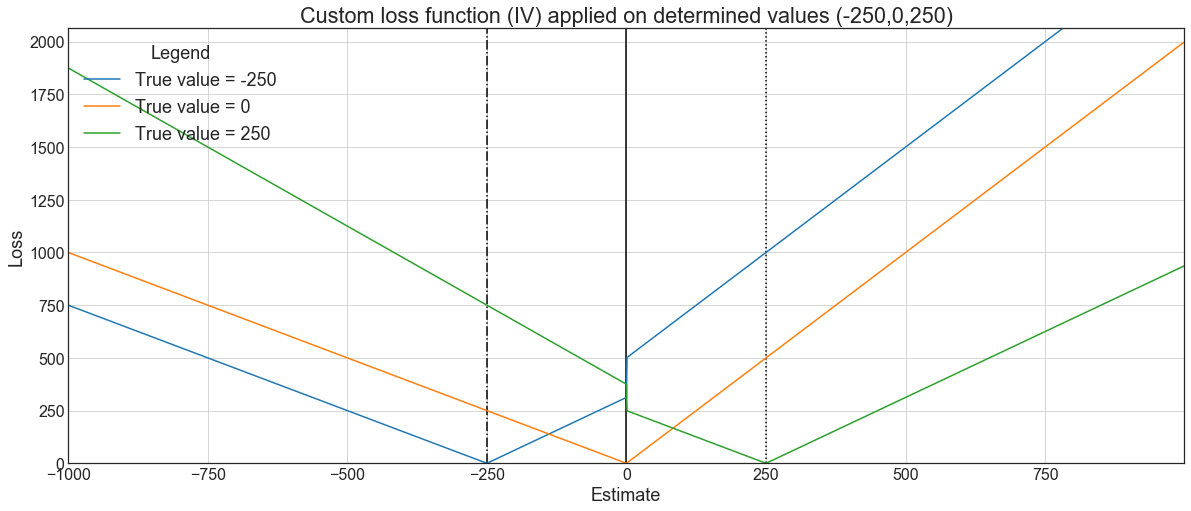
\includegraphics[width=1\textwidth]{Figures/LF4_det_values.png}
			\caption{Loss based on the customized loss function (Equation \ref{eq:LF_final}) for determined true scores of -750, 0 and 750. This plot is meant to clarify the way real losses are incurred for each guess, relative to a given true score value. The expected loss, as seen in Figure \ref{fig:LF_4steps_normal}, is acquired by arithmetically averaging such deterministic loss realizations based on the true score probability distribution by using Equation \ref{eq:ExpectedLoss2}.}\label{fig:LF4_det_values}
		\end{figure}
		
		Combining these adaption steps and the conditions defined in them, results in the following customized loss function:
		
		\begin{equation}\label{eq:LF_final}
		L(\theta,\hat{\theta}) =
		\begin{cases}
		|\theta - \hat{\theta}|, & \text{for } 0<\hat{\theta}<\theta  \\
		|\theta-\hat{\theta}|*a, & \text{for } 0<\theta<\hat{\theta} \\
		|\theta-\hat{\theta}|*b, & \text{for } \theta\leq0<\hat{\theta} \\
		|\theta-\hat{\theta}|*c, & \text{for } \hat{\theta}\leq0<\theta 
		\end{cases},
		\text{ with } a,b,c \in \mathbb{Q}.
		\end{equation}  
		It is important to note that the weighting factors defined above can take basically any numerical values but should be chosen in a way that they appropriately represent the framework conditions of the problem. Here, based on the considerations named above, it is assumed that normal overestimation is 25\% (\textit{a} = 1.25), fatal overestimation 100\% (\textit{b} = 2) and fatal underestimation 50\% (\textit{c} = 1.5) worse than normal underestimation. \\		
		It has to be emphasized that this is just one possible proposal for loss function customization. There exists not one perfect design for such a case. Slight to strong changes can already be implemented by simply varying the values of the weighting factors \textit{a, b} and \textit{c}. Fundamentally different loss functions can also be based on a significantly different mathematical structure. Loss functions are customized regarding the problem environment and according to the subjective needs and objectives of the decision maker. Thus, they are mostly defined by the actor expressing his perspective. Changes in the individual's perception and attitude might lead to further customization needs at a future point in time, as was reported by \citet{hennig2007}. Especially considering individual persons as actors, psychological aspects may play a significant role.
		
		\subsection{Including different risk-affinities in the loss function}
		
		It can be assumed that several actors in one sector or decision environment may have the same general loss function but different affinities concerning risks. This might be based for example on different psychological factors or economic philosophies followed by companies. It might also be based on budgets and options such actors have available. An intuitive example is the comparison of a small and a large company. A certain false estimate or error might have a significantly stronger impact on a company which has a a generally lower market share and only few projects, than on a larger company which might possess a higher financial flexibility and for which one project is only one of many development options in a portfolio.\\		
		In the following, the loss function is further adapted to consider different risk-affinities of several actors. Representing risk behavior in a loss function can also be done in different ways and regarding different types of risks. Here, bidding lower is considered the cautious, risk-averse option, as smaller losses can be expected from underestimating. Guessing higher is deemed riskier, as losses from overestimation are greater. However, bidding correctly on a higher value, will also return a greater gain. It is assumed that risk-friendly actors care less about fatal underestimation, i.e. they will rather develop a project than discard it. In the loss function, risk is simply included using a risk factor \textit{r} which alters the incurred losses respectively:
		\begin{equation}\label{eq:LFR_final}
		L(\theta,\hat{\theta}) =
		\begin{cases}
		|\theta - \hat{\theta}|*r^{-0.5}, & \text{for } 0<\hat{\theta}<\theta  \\
		|\theta-\hat{\theta}|*a*r, & \text{for } 0<\theta<\hat{\theta} \\
		|\theta-\hat{\theta}|*b*r, & \text{for } \theta\leq0<\hat{\theta} \\
		|\theta-\hat{\theta}|*c*r^{-0.5}, & \text{for } \hat{\theta}\leq0<\theta 
		\end{cases},
		\text{ with } a,b,c,r \in \mathbb{Q}.
		\end{equation}	
		\begin{figure}[h]
			\centering
			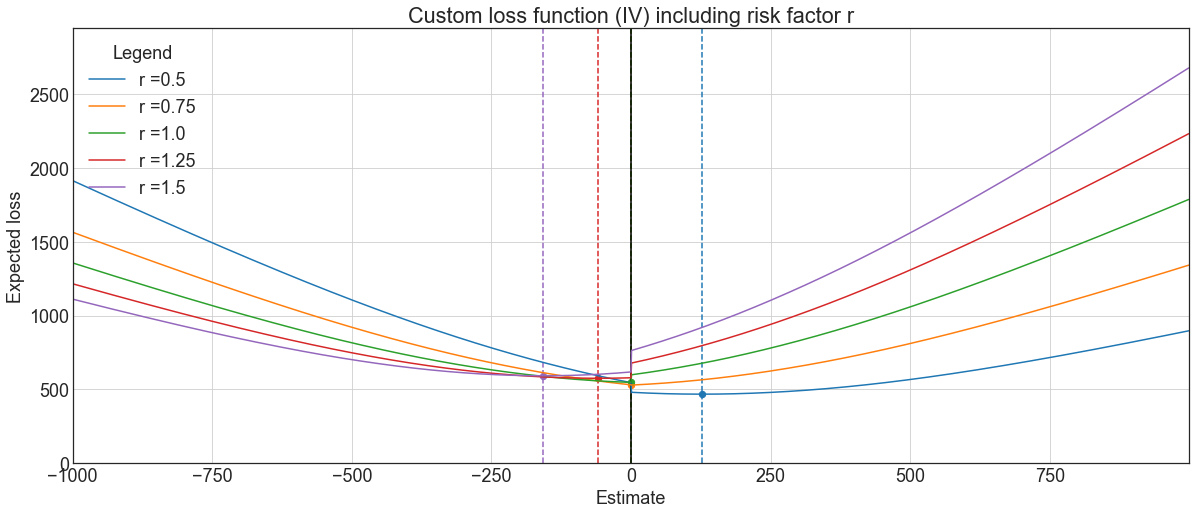
\includegraphics[width=1\textwidth]{Figures/LFR_normal2.png}
			\caption{Plotting of expected loss realizations after including the risk factor $r$ in the loss function (Equation \ref{eq:LFR_final}) for actors with risk-affinities ranging from risk-averse ($r$ = 0.5 and 0.75), over risk-neutral ($r$ = 1), to risk-friendly ($r$ = 1.25 and $r$ = 1.5). The loss function was applied on a normal distribution around zero ($\mu=0; \sigma=500$).}\label{fig:LFR_normal} 
		\end{figure}
		According to this, for \textit{r} = 1 the risk-neutral loss function is returned, as no re-weighting takes place. For \textit{r} $<$ 1, the weight on overestimating (\textit{a, b}) is reduced and increased for fatal underestimation (\textit{c}), as well as normal underestimation. This represents a risk-friendlier actor that is willing to bid on a higher estimate to attain a greater gain. For \textit{r} $>$ 1, the overestimation weight (\textit{a, b}) is increased in the loss function, underestimation and fatal underestimation weight (\textit{c}) are decreased and respectively more risk-averse actors are prompted to bid on lower estimates.\\		
		The factor \textit{r} can take basically any positive values. However, since risk-neutrality is expressed by \textit{r} = 1, values 0 $<$ \textit{r} $<$ 2 are considered to be the most appropriate choices to represent both sides of risk-affinity equally here.		
		
		\section{1D geological reservoir modeling}\label{sec:1D_model}
		For simple understanding and a preliminary assessment of the Bayesian statistical methods and the loss function described above, they are first to be applied in the context of a conceptual one-dimensional hydrocarbon system case. The underlying model and basic approach are inherited from \citet{delaVarga2016}, but the parameters are adapted to more appropriately represent a reasonable geological petroleum system, consisting of a reservoir formation with overlying seal in the subsurface. In this 1D setting, only the interface depths and thicknesses of layers such as the reservoir or seal unit can be observed. Other defining aspects, such as structural entrapment, are assumed to be given. Limiting the model to only one dimension and a small number of uncertain stratigraphical parameters allows for a relatively straightforward and simplified approach to assessing an abstract type of value for a reservoir, applying the custom loss function (Equation \ref{eq:LF_final}) for value estimation and observing respective effects of Bayesian inference. The construction of the 1D geological model is described in the following.
			\begin{figure}[h]
				\centering
				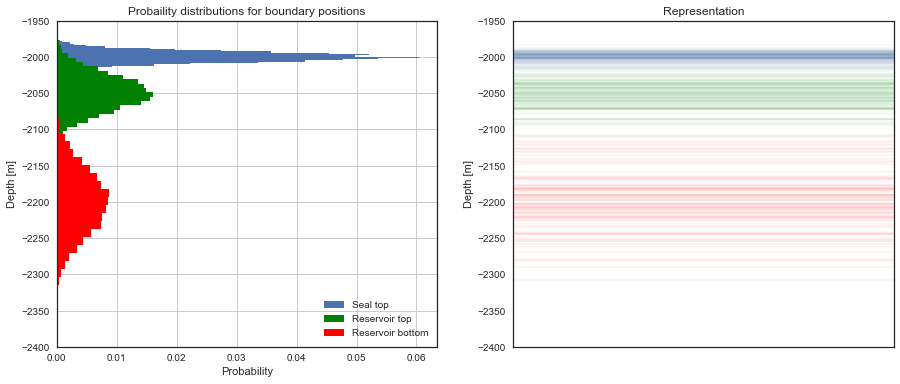
\includegraphics[width=1\textwidth]{Figures/1D_model.png}
				\caption{Probability distributions for positions of layer boundaries in the subsurface and a respective representation using lines. These normal distributions are determinedby the following values: Seal top: $\mu = 2000 m, \sigma = 7$; reservoir top: $\mu = 2050 m, \sigma = 25$; reservoir bottom: $\mu = 2200 m, \sigma = 45$. }\label{fig:1D_model}
			\end{figure}
			\subsection{Construction of the 1D geological model}\label{sec:1D_construction}	
			\citet{delaVarga2016} constructed a simple geological model using three uncertain positions in vertical one-dimensional space, marking hypothetical boundaries of layers in a subsurface column. The location probabilities for these points are defined by sampling from normal distributions. These points confine two layers in the middle, from which the upper one can be labeled as seal and the lower one as reservoir. The standard deviations ($\sigma$) of the distributions increase with depth, representing an increase in uncertainty. For an approximate representation of a hydrocarbon reservoir system, the distribution means ($\mu$) are set to depths of 2000 m (seal top, $\sigma=7$), 2050 m (reservoir top, $\sigma=25$) and 2200 m (reservoir bottom, $\sigma=45$). The resulting model with its prior distributions of possible layer boundary locations is illustrated in Figure \ref{fig:1D_model}.
			%\begin{figure}[h]
			%\centering
			%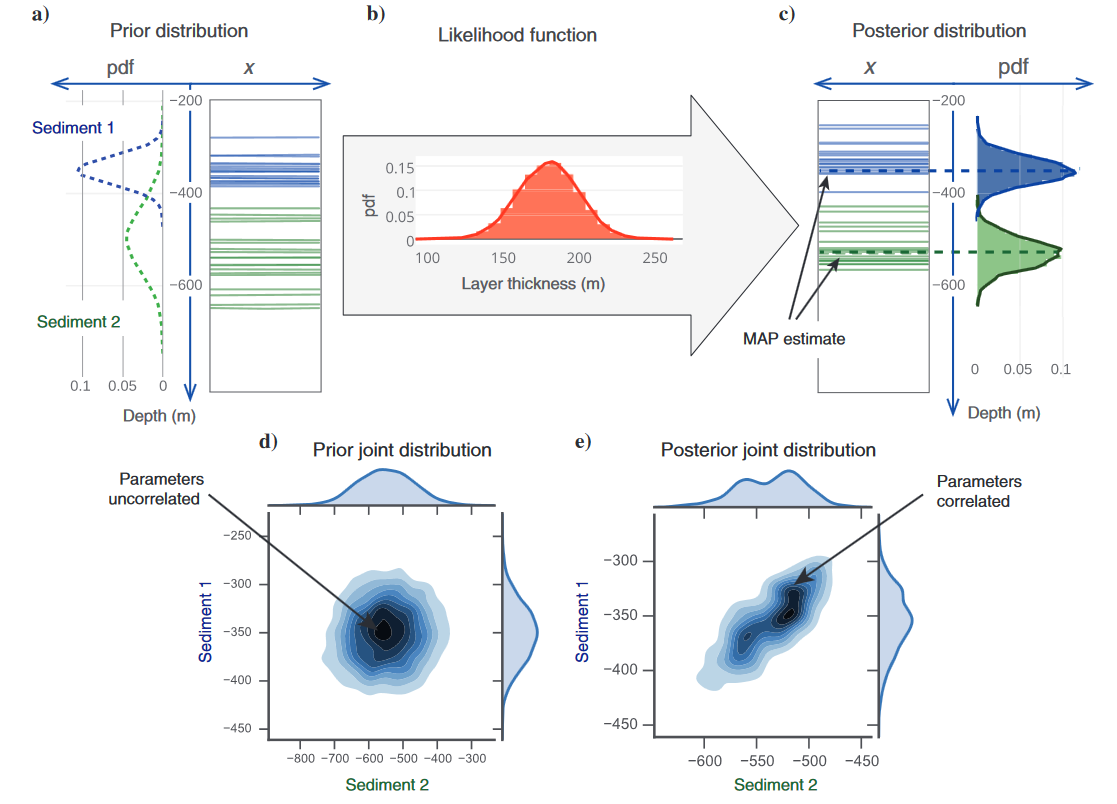
\includegraphics[width=1\textwidth]{Figures/1D_principle.PNG}
			%\caption{Conceptual illustration of applying Bayesian inference in an abstract 1D geological model as conducted by \citet{delaVarga2016}. Prior distributions of layer boundaries in depth (a) are updated using thickness likelihoods (b) to attain posterior distributions (c). Model parameters which are uncorrelated in their joint probability distribution before the inference (d), are correlated after performing Bayesian inference (e) (from \citet{delaVarga2016}).}\label{fig:1D_principle}
			%\end{figure}
			%\subsection{Bayesian inference and analysis of the 1D case}\label{sec:1D_bayes}
			For conducting Bayesian inference, it is assumed that new observations are made, providing additional information considered here in the form of likelihood functions for the thicknesses of the two layers of interest. Likelihood functions for reservoir and seal thicknesses are introduced based on another set of normal probability distributions. These are directly related to the layer boundary positions, i.e.\ the prior parameter distributions. Means and standard deviations of the likelihood distributions are variable, so that several scenarios based on the assumption of different observations can be tested. Parameter priors and likelihood functions are embedded into a probabilistic modeling framework as described in Section \ref{sec:numerical_implementation} and MCMC sampling is conducted accordingly. Performing Bayesian inference on such a 1D geological model follows the conceptual example devised by \citet{delaVarga2016}. Posterior distributions are to be evaluated based on the valuation method described in the following.
			
	        \subsection{Abstract valuation of the 1D geological model}\label{sec:1D_score_system}
	        For valuating a simplified 1D model, $OOIP$ and recoverable volume calculations are not applicable, as these require a 3D setting. Given only layer boundary positions in one vertical dimension, it is resorted to an abstract way of reservoir valuation by defining a scoring system. A dimensionless reservoir score is made dependent on three derivatives of the uncertain 1D interface positions: (1) reservoir thickness, (2) reservoir top depth and (3) seal thickness. From these, (2) equals the prior parameter that indicates the reservoir-seal boundary in depth. The other two are respectively deduced from the distance between parameter values. According to this dependence, these values, which we use to valuate the reservoir, inherit the uncertainty from their parent parameters. An exemplary comparison between the distribution of these values depending on prior and posterior parameters is depicted in Figure \ref{fig:3_parameters}. We hereby illustrate how model uncertainties are translated to uncertainties related to valuation measures.\\
	        \begin{figure}[h]
	        	\centering
	        	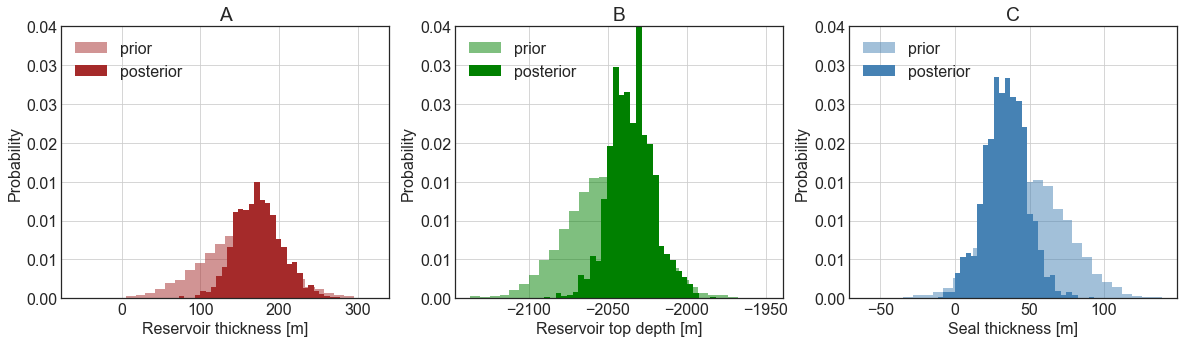
\includegraphics[width=1\textwidth]{Figures/3_parameters.png}
	        	\caption{Probability distributions for the three factors used in the abstract reservoir valuation as formulated in Equation \ref{eq:1D_score_system}. These are deduced from the 1D model input parameters and are thus uncertain. Here, we show factors deduced from prior parameters in Figure \ref{fig:1D_model} and factors resulting from exemplary posterior parameter distributions.}\label{fig:3_parameters}
	        \end{figure}
	        Assuming that reservoir thickness is a simplified indicator for the amount of extractable oil or gas and thus value in place, a gain in score can be correlated with increase in thickness. Here, two score points are assigned to one meter of thickness. Increasing costs of drilling are indicated by increasing depth of the reservoir top. Consequently, one negative score point is ascribed to every meter in depth. Samples from the probability distributions of these two parameters are drawn to model the true score of the reservoir (depth scores are subtracted from reservoir thickness scores).
	        A third parameter is defined by the seal thickness. Score points are not added or subtracted by this parameter directly. Instead, a threshold for seal reliability is defined beforehand. Here, it is set to 20 m thickness. If the seal thickness falls below this threshold, it is assumed that the seal fails completely and thus all the potential value (positive score) of the reservoir is lost, while costs of depth (negative score) remain. Thus, a condition to check whether the seal is reliable is included in the model. A respective equation for the reservoir score $S_{res}$ is defined as:
			
			\begin{equation}\label{eq:1D_score_system}
			S_{res} = 
			\begin{cases}
			2h_{res} + d_{res}, & \text{for } h_{seal} >= 20  \\
			d_{res}, & \text{for } h_{seal} < 20
			\end{cases},
			\end{equation}
			
			where reservoir thickness is given by $h_{res}$, seal thickness by $h_{seal}$ and reservoir depth, which is always a negative value, by $d_{res}$.\\
			This valuation method is applied on the original prior-only Monte Carlo simulation of the 1D model as reference and then on each posterior distribution set after conducting Bayesian inference. Resulting score probability distributions can be compared directly and additionally under use of the case-specific custom loss function (Equation \ref{eq:LFR_final}) defined before. 
		
		\section{3D geological reservoir model}\label{sec:3D_model}
		The concept of the 1D geological model is to be transferred and extended to a 3D setting that incorporates a more realistic and complete geological reservoir system. A three-dimensional space allows not only for better consideration of stratigraphical aspects, but also for the inclusion of structural formations, in particular hydrocarbon trap-defining features.
		
		\subsection{Design of the 3D geological reservoir model}\label{sec:3D_design}
		For the purpose of exploring the application and effects of Bayesian analysis and decision theory in this work, the model is nevertheless to be kept conceptual and relatively simple. Stratigraphically, it is designed to include one main reservoir unit (sandstone), one main seal unit (shale), an underlying basement through which hydrocarbon fluids could have flown upwards and overlying formations that are assumed to be permeable, so that hydrocarbons can escape upwards. Structurally, it is constructed to feature an anticlinal fold that is displaced by a normal fault. All layers are tilted so that they dip in the opposite direction of the fault plane dip. The original concept of this model is designed in a way that a potential hydrocarbon trap is formed in the reservoir rock enclosed by the deformed seal and the normal fault.\\
		This trap, more specifically the trap volume, is defined as the central feature of economic interest. For conducting simple and straightforward volumetric calculations, it is assumed that found closed traps are always filled to spill with oil, i.e. the complete trap volume is hydrocarbon filled and the $OOIP$ can be attained over this volume.\\
		The maximum trap volume is assumed to equate the hydrocarbon-filled rock volume $A * h$ in Equation \ref{eq:OOIP} and is thus to be used to valuate each realization of the geological model. Single results are expected to vary, depending on the uncertain input parameters defined in Section \ref{sec:3D_construction} below. The custom loss function \ref{eq:LFR_final} is to be applied on the resulting value distributions before and after performing Bayesian inference. This way, the effect of incorporating additional information in the form of likelihoods is to be assessed from a perspective of Bayesian decision theory. It is furthermore assumed that the hydrocarbon trap volume is directly linked to a project development decision, i.e. investment and allocation of resources is represented by bidding on a volume estimate.
		
		\subsection{Construction of the uncertain 3D geological reservoir model}\label{sec:3D_construction}
		The 3D structural geological model is constructed as follows: In principle, it is defined as a cubic block with an extent of 2000~m in X, Y and Z directions. The basic input data for the interpolation of the geological features is comprised of 3D point coordinates for layer interfaces and fault surfaces, as well as measurements that indicate respective dip directions and angles. In a Python environment, the data is imported as comma-separated values (CSV) using GemPy. From the generated data frame, GemPy is able to interpolate surfaces following the potential-field method explained in Section \ref{sec:struc_geo_modeling} and compute voxel-based 3D geological models (see Figure \ref{fig:3Dmodel_construction}).
		\begin{figure}[h]
			\centering
			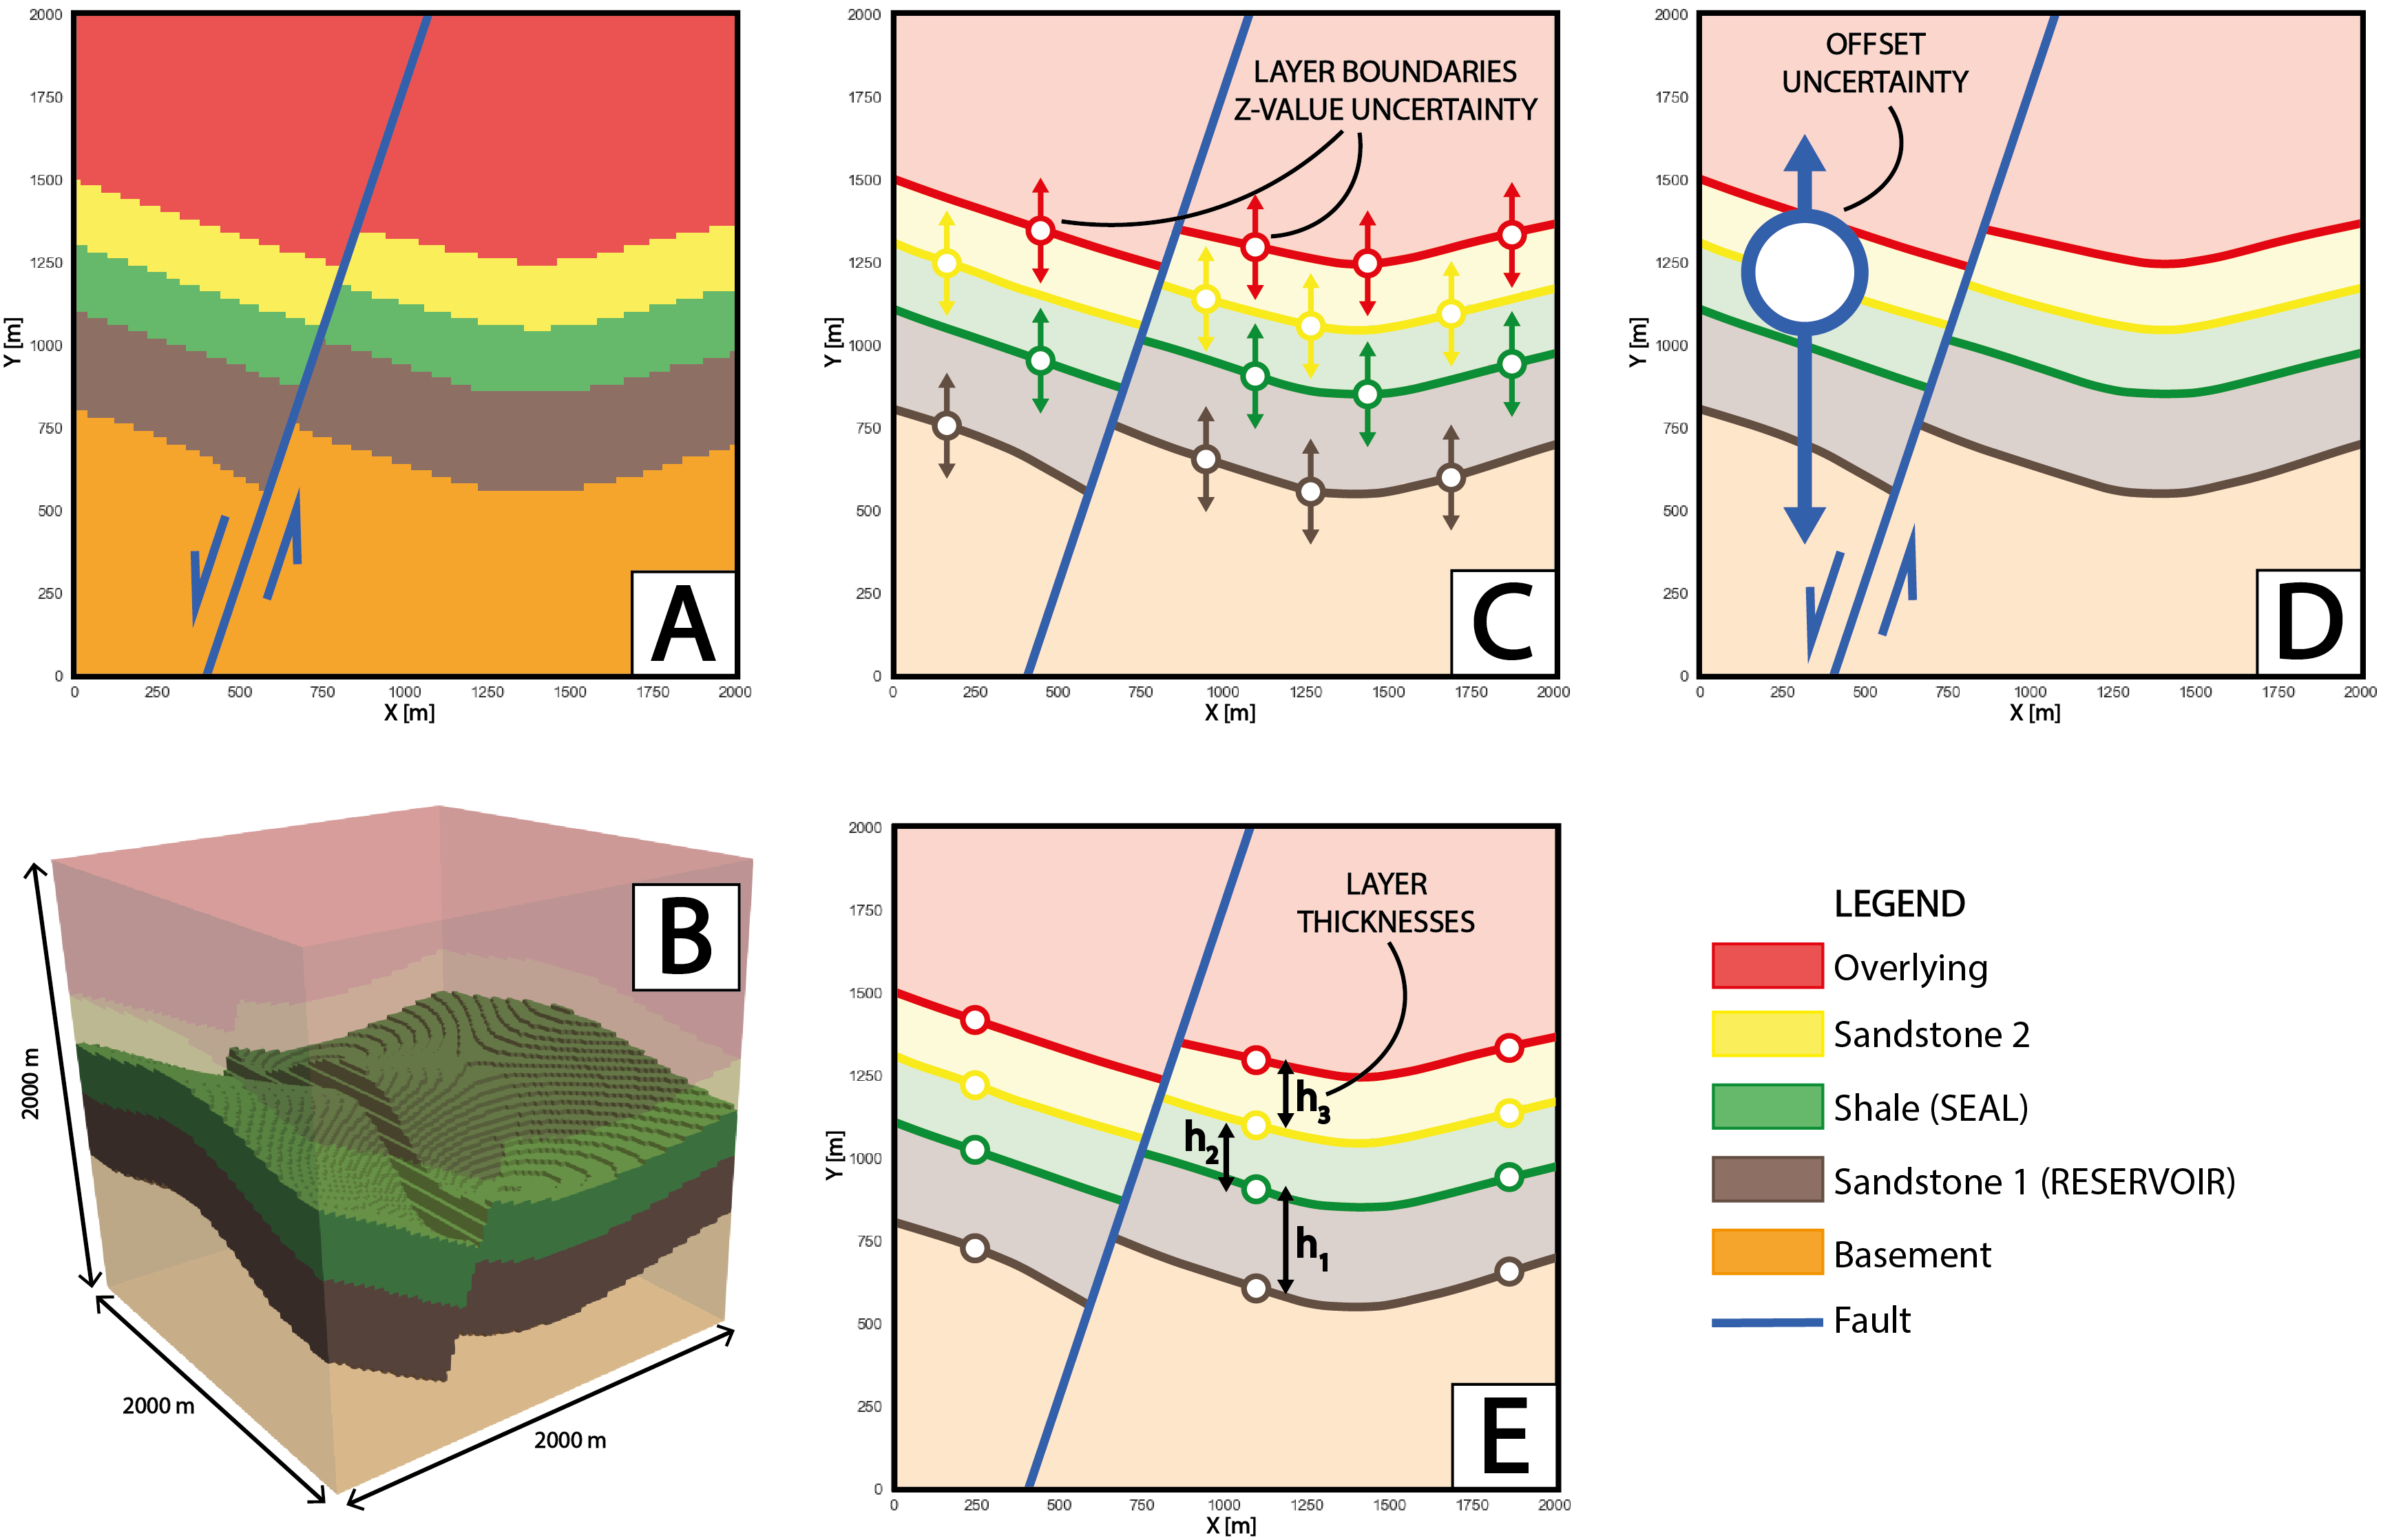
\includegraphics[width=1\textwidth]{Figures/Uncertainties_Likelihoods.png}
			\caption{Illustration of the design and construction of the 3D structural geological model. A 2D cross section through the middle of the model, perpendicular to the normal fault, is shown in (A). A 3D representation of the model, highlighting the reservoir and seal formations as voxels, is visualized in (B). In (C) and (D), the inclusion of parameter uncertainties is presented. Colors indicate certain layer bottoms (i.e. boundaries) which are assigned a shared normal distribution on which their z-positional uncertainties are based (C). All points in the hanging wall are additionally assigned a fault offset uncertainty based on a skew normal distribution (D). Thicknesses of the three middle layers are defined by the distances of boundary points (E) and are thus directly dependent on (C). These thicknesses are to be defined as likelihoods.}\label{fig:3Dmodel_construction}
		\end{figure}
		This model allows for the consideration of various kinds of uncertainties and their implementation in several different ways. Here, they are included by assigning uncertainties to the Z-positions of points which mark layer tops and interfaces in the 3D space. This is achieved based on respective probability distributions from which deviation values are drawn, which are then added to the original input data Z-value. Uncertainties regarding layer surface positions in depth, layer thicknesses, topological shape and degree of fault offset can be incorporated. These can be assigned as homogeneous sets to groups which are to share a common degree of uncertainty. Here, points belonging to the same layer interface are assigned the same base uncertainty by applying one shared probability distribution. Assuming an increase of uncertainty with depth, standard deviations for the distributions are increased for lower formations. Furthermore, uncertainty regarding the magnitude of fault offset is incorporated by adding a skew normal probability distribution that is shared by all layer interface points on the hanging wall. A left skewed ($\alpha=-2$) normal distribution is chosen to reflect the nature of throw on a normal fault, particularly the slip motion of the hanging wall block. Mainly negative values are returned by this distribution. This way, the offset nature of the normal fault is maintained and the inversion to a reverse fault is avoided. Specific ditributions used to represent uncertainties are listed in the Appendix.
		%\begin{enumerate}
		        %\item \textbf{Z-values for layer interfaces:} Analogously to the 1D model, uncertainties for the vertical position of layer interfaces are implemented by using normal probability distributions. A deviation from the original input data Z-value is hereby added and allows for the consideration of uncertainties regarding layer surface positions in depth, layer thicknesses, topological shape and degree of fault offset. Points belonging to the same layer interface are assigned the same base uncertainty by applying one shared probability distribution. Assuming an increase of uncertainty with depth, standard deviations for the distributions are increased for lower formations. Furthermore, uncertainty regarding the magnitude of fault offset is incorporated by adding a further normal probability distribution that is shared by all layer interface points on the hanging wall. The specific ditributions are listed in the Appendix.
		        %\item \textbf{Cross-fault sealing:} Uncertainty about the sealing capacity across the fault is implemented using a Bernoulli distribution. In doing so, a probability of success is defined beforehand. In the case of such a "success", a value of one is returned by the distribution and lateral sealing of the fault is assumed. Should a value of zero be returned, cross-fault leakage is determined to be generally possible, depending on the occurrence of juxtapositions.
		        %\item \textbf{Other non-structural parameters:} Other factors that determine the $OOIP$ and $ROV$ calculations, such as porosity and recovery factor, can be implemented stochastically or deterministically. WHAT DO I USE?
		%\end{enumerate}
		
		\subsection{Determination of the trap volume}
		In the course of this work, several algorithms are developed within the Python environment, that in combination enable the automatic recognition and calculation of trap volumes in geological models computed by GemPy. To assign voxels of the model to the trap volume, it is checked whether the following conditions (illustrated in Figure \ref{fig:trap_recognition}) are satisfied by each particular voxel: 
		\begin{figure}[p!]
			\centering
			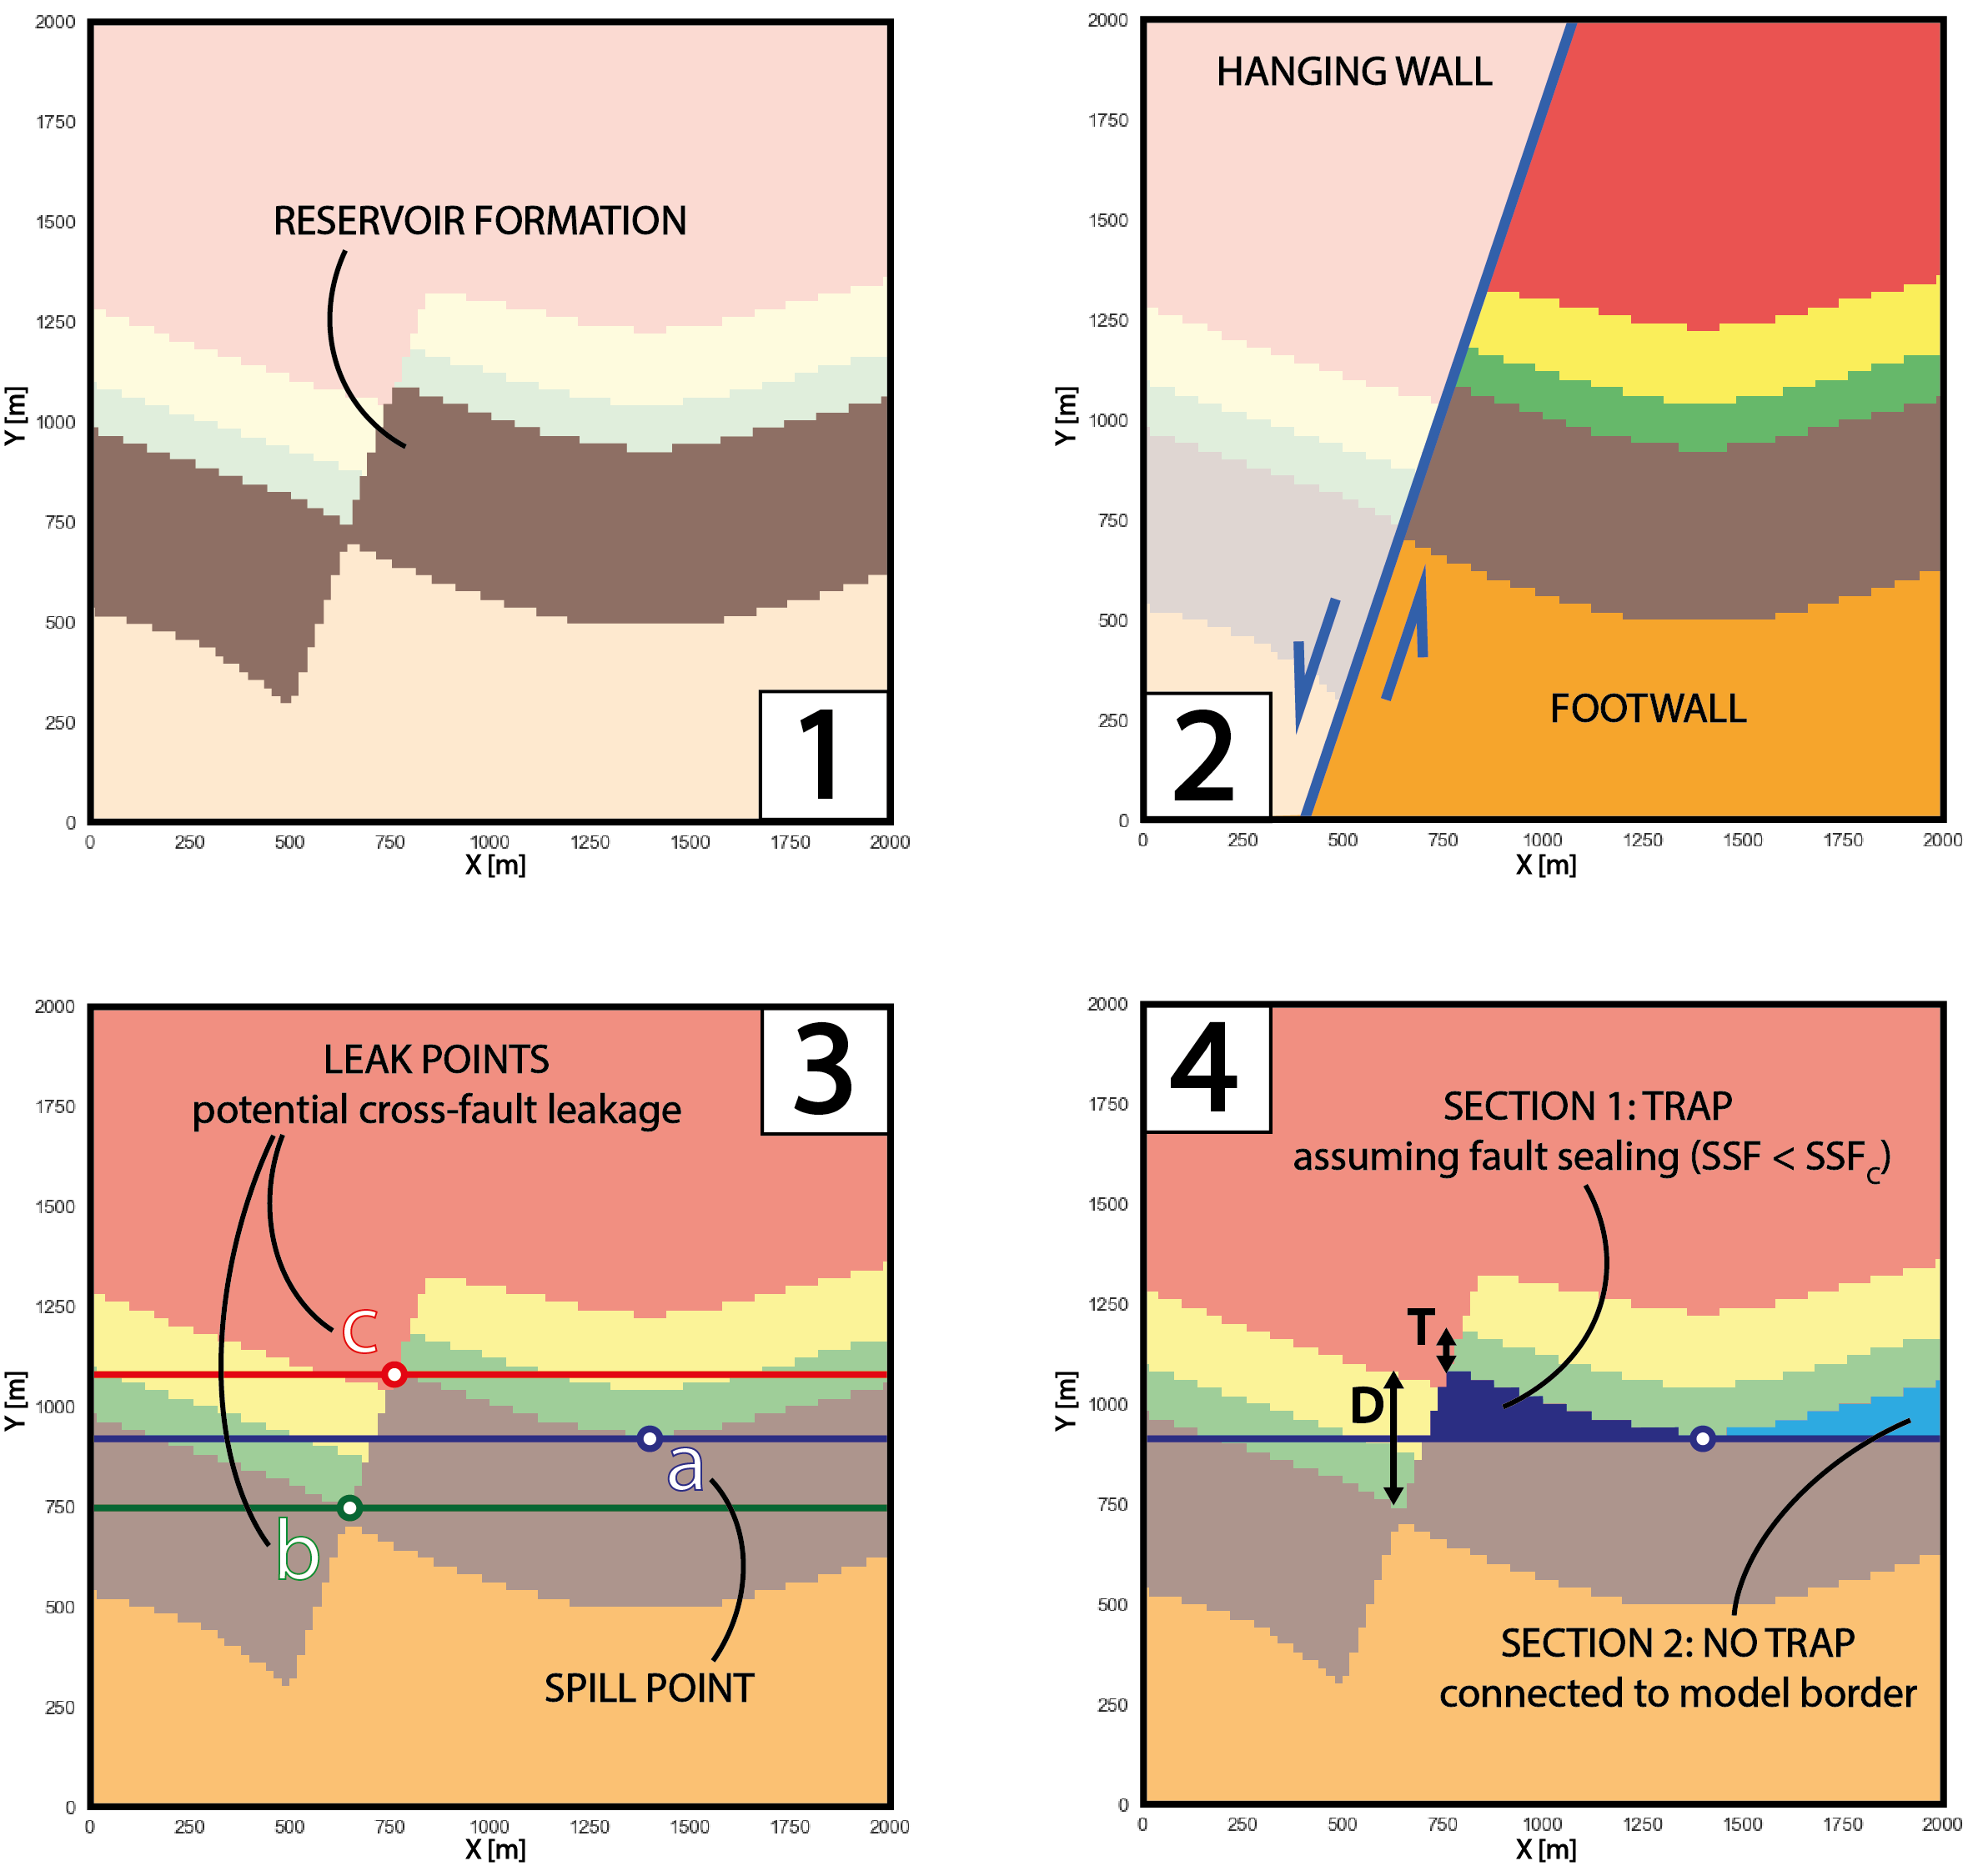
\includegraphics[width=1\textwidth]{Figures/Trap_Cond_H.png}
			\caption{Illustration of the process of trap recognition, i.e. the conditions that have to be met by a model voxel, to be accepted as belonging to a valid trap. A voxel has to be labeled as part of the target reservoir formation (1) and positioned in the footwall (2). Trap closure is defined by the seal shape and the normal fault (3). Consequently, the maximum trap fill is defined by either the anticlinal spill point (3;a) or a point of leakage across the fault, depending on juxtapositions with layers underlying (3;b) or overlying the seal (3;c). The latter is only relevant if the critical Shale Smear Factor is exceeded, as determined over $D$ and $T$ in (4). In this example, assuming sealing of the fault due to clay smearing, the fill horizon is determined by the spill point in (4). Subsequently, only trap section 1 is isolated from the model borders in (4) and can thus be considered a closed trap.}\label{fig:trap_recognition}
		\end{figure}
		\begin{enumerate}
			\item \textbf{Labeled as reservoir formation:} The voxel has been assigned to the target reservoir formation (see Sandstone 1 in Figure \ref{fig:trap_recognition} (1)) in the lithology block model. This is determined by respective labeling of the input data and the computation conducted by GemPy.
			\item \textbf{Location in footwall:} The voxel is located on the footwall side of the fault. This condition is applicable to this specific model design, in which entrapment is assumed to occur between the footwall anticlinal enclosure and the normal fault. Due to respective dip of the reservoir formation, full leakage is assumed for the reservoir formation in the hanging wall. A distinction between foot- and hanging wall is easily achievable by using the fault model block that is generated by GemPy. In this fault block, voxels on both sides are assigned respective values for distinction.
			\item \textbf{Location above spill point horizon:} The voxel is located vertically above the final spill point of the trap. In the algorithm to find this final spill point, it is distinguished between a spill point defined by the folding structure, referred to as anticlinal spill point, and a cross-fault leak point, that depends on the magnitude of displacement and the resulting nature of juxtapositions. Once both of these points have been determined, the higher one is defined to be the final spill point used to determine the maximum fill capacity of the trap.  Given a juxtapostion with layers overlying the seal, due to fault displacement, the respective section is checked for fault sealing by taking into account the Shale Smear Factor value. In the case of a suitable $SSF$ and consequent fault sealing, leakage across this type of juxtaposition is discarded as irrelevant. The processes of finding the decisive spill point, as well as the determination of juxtapostions and $SSF$ is explained below in further detail.
			\item \textbf{Location inside of closed system:} The voxel is part of a model section inside of the main anticlinal feature. All of the voxels inside this particular section are separated from the borders of the model by voxels that do not meet the conditions above, which primarily means that they are encapsulated by seal voxels laterally and upwards. This condition is applicable  under the assumption, that connection to the borders of the model lead to leakage. A trap is thus defined as a closed system in this model and trap closure is assumed to be void outside of the space of information, i.e. the model space.	
		\end{enumerate}
		It has to be emphasized that these conditions have been fitted to the geological model constructed as described in Section \ref{sec:3D_construction}. For other models featuring different geological properties, features and levels of complexities, these conditions might not apply at all or might have to be adapted. Models of higher complexities will surely require the introduction of further conditions.
		
			\subsection{Finding the decisive spill or leak point of a trap} %\label{sec:spill_leak_finding}
			Regarding anticlinal structures and traps, it can be observed that, geometrically and mathematically, a spill point is a saddle point of the reservoir top surface in 3D. This was described by \citet{collignon2015fold_linkage}, who pointed out that the linkage of folds is given by saddle points. These are thus a controling factor for spill-related migration from respective structural traps. For anticlinal traps, closure can consequently be defined as the distance between the saddle point (i.e. spill point) and maximal point of the trap \citep{collignon2015fold_linkage}.\\
			Regarding a surface defined by $f(x,y)$, a local maximum at $(x_0,y_0,z_0)$ would resemble a hill top \citep{guichard2013calculus}. Local maxima will be found looking at the cross-sections in the planes $y = y_0$ and $x = x_0$. Furthermore, the respective partial derivatives (i.e. gradients) $\frac{\delta z}{\delta x}$ and $\frac{\delta z}{\delta y}$ will equal zero at $x_0$ and $y_0$, i.e. that the extremum is a stationary point \citep{guichard2013calculus, weisstein2017saddlepoint}. In the context of a geological reservoir system, such a hill can be regarded as a representation of an anticlinal structural trap. Local minima are defined analogously, presenting local minima in both planes at a stationary point \citep{guichard2013calculus}. A saddle point, however, is a stationary point, while not being an extremum \citep{weisstein2017saddlepoint}. In general, saddle points can be distinguished from extrema by applying the second derivative test \citep{guichard2013calculus, weisstein2017saddlepoint}: Considering a 2D function $f(x,y)$ with continuous partial derivatives at a  point $(x_0,y_0)$, so that $f_x(x_0,y_0) = 0$ and $f_x(x_0,y_0) = 0$, the following discriminant $D$ can be introduced:
			\begin{equation}\label{eq:discriminant_D}
			D(x_0,y_0) = f_{xx}(x_0,y_0)f_{yy}(x_0,y_0) - f_{xy}(x_0,y_0)^2.
			\end{equation}
			Using this, the following holds for a point $(x_0,y_0)$:
			\begin{enumerate}
				\item If $D > 0$ and $f_{xx}(x_0,y_0) < 0$, there is a local maximum.
				\item If $D > 0$ and $f_{xx}(x_0,y_0) > 0$, there is a local minimum.
				\item If $D < 0$, there is a saddle point at the point $(x_0,y_0)$.
				\item If $D = 0$, the test fails \citep{guichard2013calculus}.
			\end{enumerate}
			\begin{figure}[h]
				\centering
				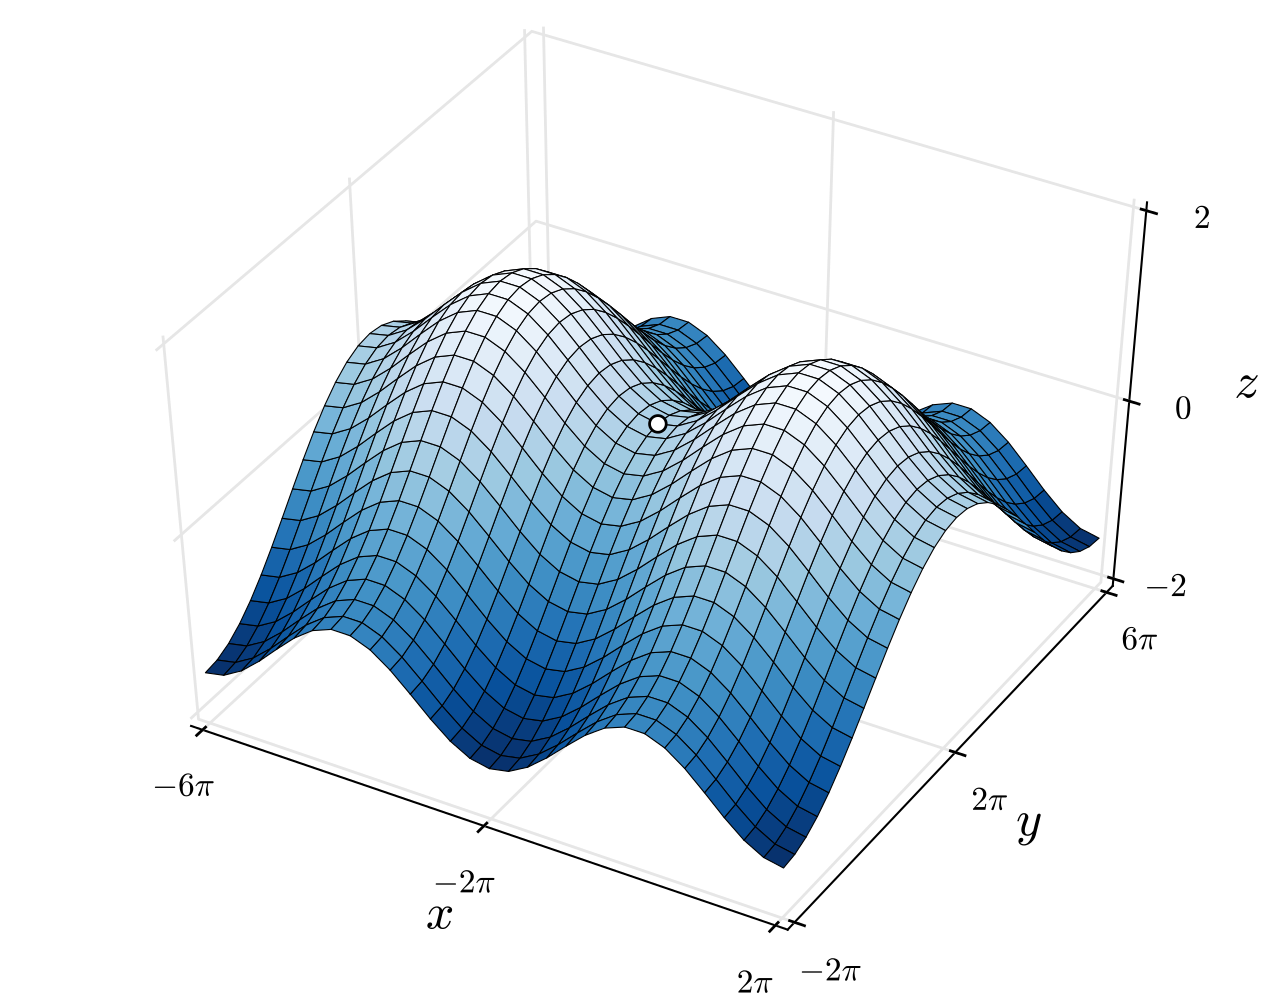
\includegraphics[width=1\textwidth]{Figures/Saddle_Point_between_maxima.png}
				\caption{Saddle point (red dot) between two maxima. In a geological setting, these surface maxima may be interpreted as two dome-shaped four-way closure traps. Spill-related migration between the two structures would take place over the saddle point, i.e. the spill point.}\label{fig:saddle_point_maxima}
			\end{figure}
			%\begin{figure}[h]
			%	%\centering
			%	\begin{subfigure}{.5\textwidth}
			%	\centering
			%	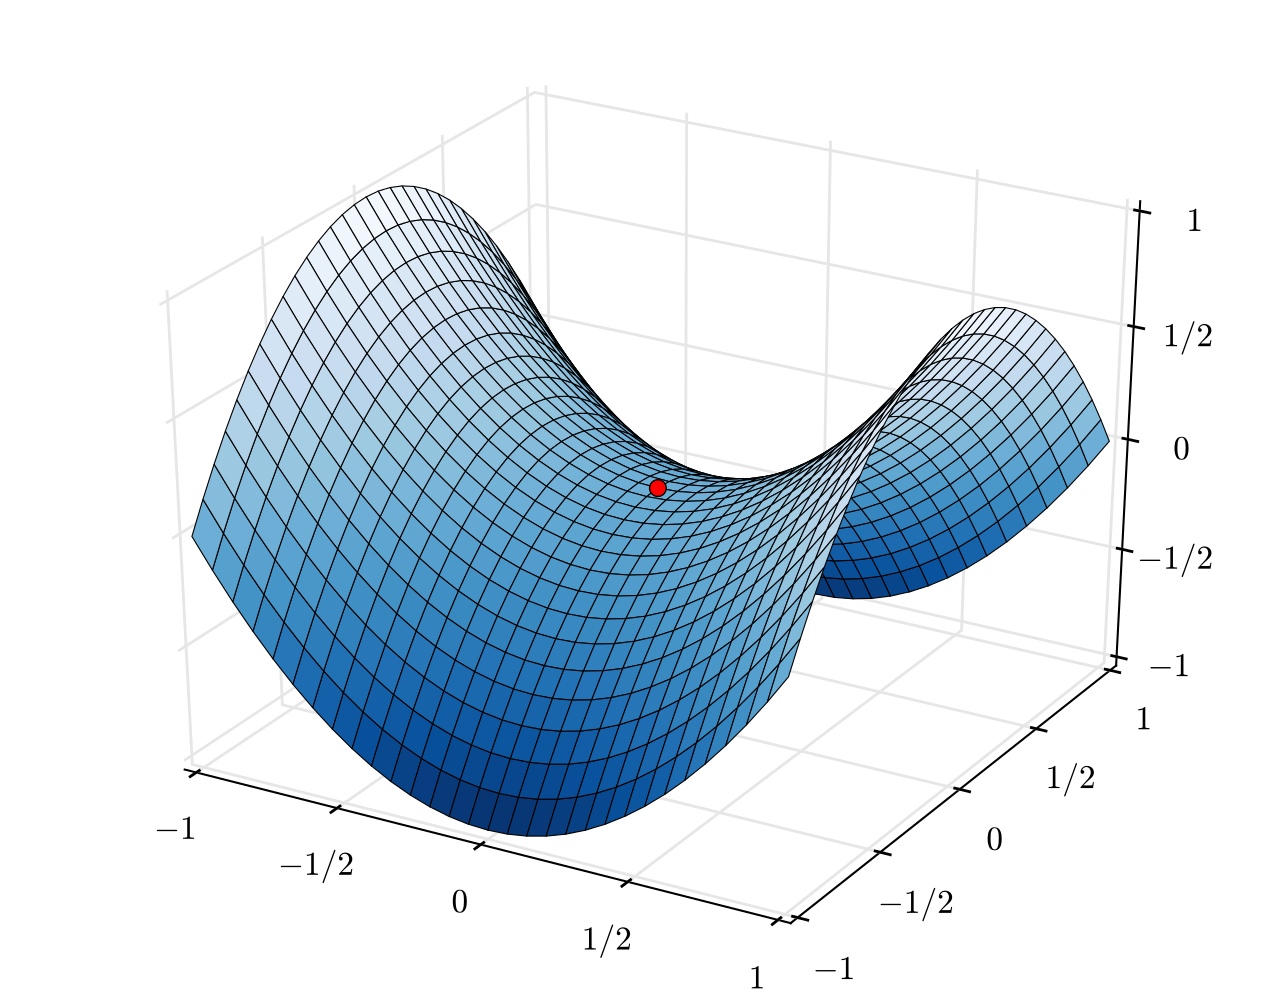
\includegraphics[width=1\linewidth]{Figures/Saddle_point.png}
			%	\caption{Graph and saddle point of the function $z=x2~-~y2$.}\label{fig:saddle_point} 
			%\end{subfigure}
			%	\begin{subfigure}{.5\textwidth}
			%	\centering
			%	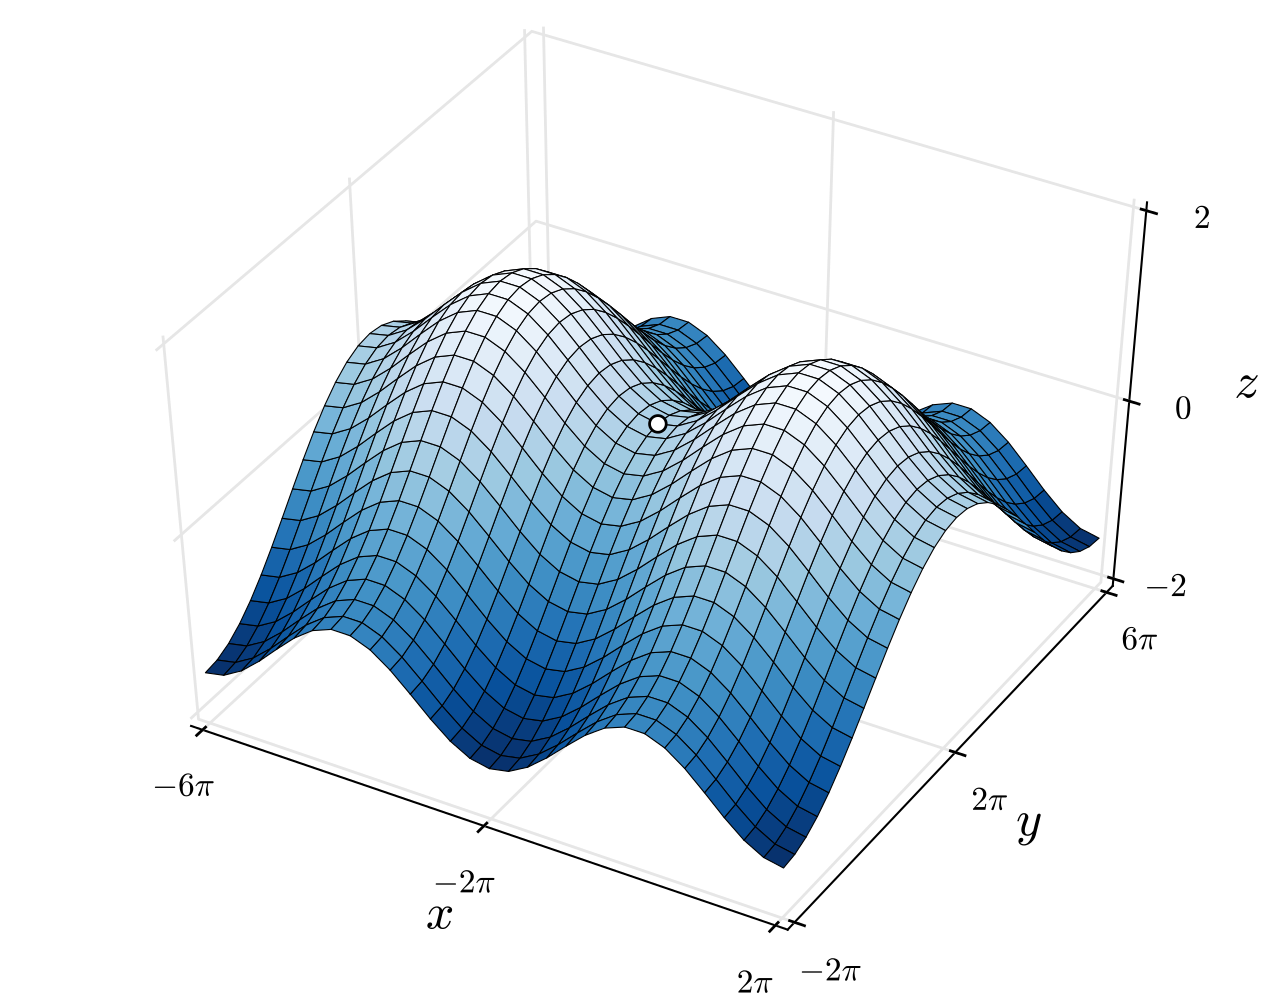
\includegraphics[width=1\linewidth]{Figures/Saddle_Point_between_maxima.png}
			%	\caption{Saddle point between two maxima.}\label{fig:saddle_point_between_maxima} 
			%	\end{subfigure}
			%	\caption{Two examples for saddle points on surfaces of 3D functions (from Wikimedia Commons)}\label{fig:saddle_points_general}
			%\end{figure}		
			Figure \ref{fig:saddle_point_maxima} can be seen as a representation of a point of spill between two dome structures (i.e. surface maxima or "hills") which is defined by the surface's saddle point between both.\\			
			In GemPy, layer boundary surfaces are returned in the form of discretized arrays of simplices and vertices. The latter can be interpolated to a 2D rectangular grid that contains Z-positional values for the surface in X and Y directions. According to \citet{verschelde2017programmingtools}, a saddle point in a matrix is maximal in its row and minimal in its column. This corresponds to the logical geometrical deduction, that a saddle point for a surface defined by $f(x,y)$ is marked by a local maximum in one plane, but a local minimum in the perpendicular plane. This is observable in Figure \ref{fig:saddle_point_flow} and made use of in the respective algorithm in this work.
			\begin{figure}[h]
				\centering
				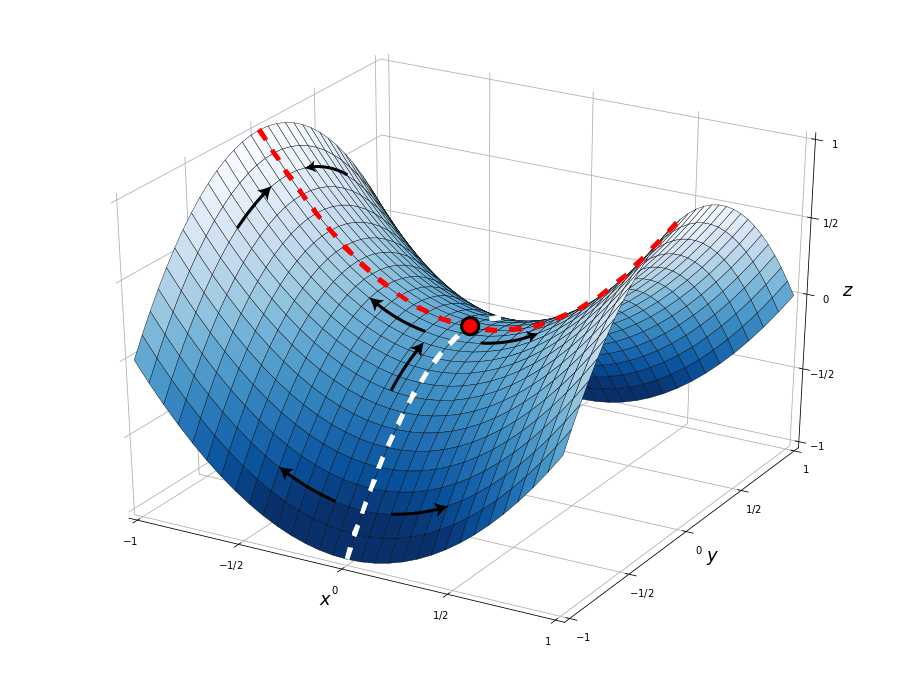
\includegraphics[width=1\textwidth]{Figures/Saddle_point_flow}
				\caption{Surface and saddle point (red dot) generated by the function $z=x2~-~y2$. Maxima in direction $y$ is marked by a red, minima in direction $x$ by a white dashed line. Considering the surface as a seal, consequent buoyant flow directions are indicated by arrows. Such flow would be directed away from minima and towards maxima, with the saddle point indicating a junction and divide, i.e. a possible spill point.}\label{fig:saddle_point_flow}
			\end{figure}
			%Regarding leakage across the normal fault in this geological model, a similar approach is taken. If the fault offset remains small enough, that the seal layer is not broken, then the reservoir top surface can be used to find the cross-fault leak point. In this case, the leak point can be defined as the maximal point of hanging wall contact of the reservoir top surface with the fault. At the same time, this point will be a local minimum on the plane perpendicular to the normal fault and thus equal a saddle point. However, higher magnitudes of fault displacement can lead to breaking of the seal, i.e. the juxtaposition of the trap structure with overlying formations which are assumed to be complete permeable. In this case, the maximum footwall contact of the surface with the fault is to be defined as cross-fault leak point.\\
			Regarding leakage across the normal fault in this geological model, a similar approach is taken. The reservoir top surface can be used to find the cross-fault leak point regarding juxtapositions with layers underlying the seal. In this case, the leak point can be defined as the maximal point of the hanging wall contact of the reservoir top surface with the fault. At the same time, this point will be a local minimum on the plane perpendicular to the normal fault and thus equal a saddle point. Higher magnitudes of fault displacement can lead to detachment of the seal in the hanging wall and consequently the juxtaposition of the trap section with seal-overlying formations which are assumed to be completely permeable. This case is dealt with independently, by checking this area of juxtaposition with regard to its $SSF$ and potential fault sealing, as is further elaborated in Section \ref{sec:check_juxta} below.\\
			Following these observations, the algorithm developed in this work uses differentiation techniques to find local extrema in the 2D reservoir top surface arrays attained over GemPy. Points where local minima and maxima of perpendicular axes X and Y coincide are then defined as saddle points. The anticlinal spill point is deduced as the maximal saddle point in the footwall. The cross-fault leak point is determined analogously in the hanging wall. In the end, whichever point of these two is maximal, is defined to be the decisive spill point of the trap. If no cross-fault leak point is found, it is presumed that full leakage is allowed to take place due to little or no displacement of the reservoir layer. Given only minor fault offset, no local maximum is found in the plane perpendicular to the fault. The Z-value of the decisive spill point is used to determine the maximum down-to-horizon to which the trap feature can be filled.
			%However, if fault sealing is given, any fault leakage and respective leak points become irrelevant and only the anticlinal spill point is considered.
			%\begin{figure}[h]
			%	\centering
			%	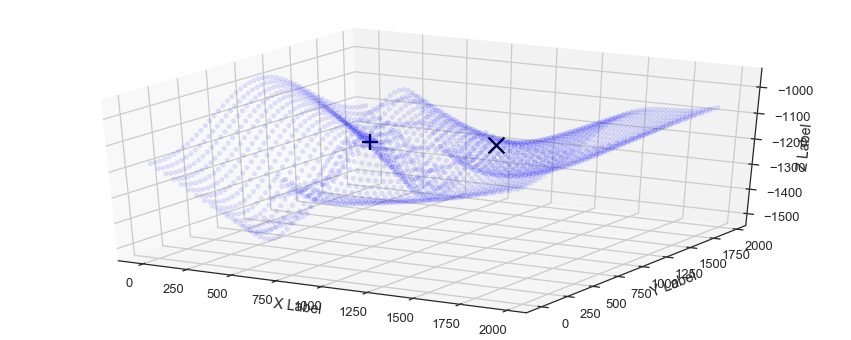
\includegraphics[width=1\textwidth]{Figures/restop_surface_spill_leak.png}
			%	\caption{Plot of reservoir top surface points and determined anticlinal spill point (marked by 'X') and cross-fault leak point (marked by '+').}\label{fig:restop_surface_spill_leak}
			%\end{figure}\\	
			\citet{kuijper2004detecting} has pointed out that finding spatial critical points, saddle points especially, can be problematic using discretized methods and rectangular grids in particular. Finding all extrema and saddle points can be difficult \citep{kuijper2004detecting}. Failures to detect saddle points in this work's model are resolved by adding a buffer around extrema that define the anticlinal structure. However, it has to be pointed out that saddle points might still be missed in some rare cases, especially if they are located in an orientation which is "rotated" and not aligned with the X and Y axes. Furthermore, in this work, the geological model is designed in a way that saddle points are presumed to only occur within or near the structures of interest and are thus easier to differentiate.
						
			\subsection{Checking for juxtapositions and possible fault sealing}\label{sec:check_juxta}
			Given a juxtaposition of a trap section with layers overlying the seal across the fault, the respective area is to be examined with regard to its clay smearing potential. Here, this is achieved by calculating the $SSF$ as introduced in Section \ref{sec:Reservoir_values}. Juxtaposition areas can be attained using a topology function that is part of GemPy. On the base of this, a new function is created, with which the Z-extent, i.e. the height of relevant juxtapositions can be deduced. These are juxtapositions of all layers on which the seal slipped and seal-overlying formations. In the case of high displacement, for example, the footwall reservoir, but also the basement might be in contact with units above the seal in the hanging wall. The  heights of each of these single juxtapositions, below the point of maximum displacement at the trap, are added up to attain a total juxtaposition height. Consequently, the fault throw can be attained by adding the seal thickness to this. The resulting displacement value can then be related to the seal thickness to obtain the Shale Smear Factor.\\
			As mentioned before, it has been reported that the critical value $SSF_c$ is dependent on scale and can expected to be lower with larger shale thicknesses and greater fault throws. So, as the scale in the present geological model is relatively large, but also for the purpose of shedding light on different conceptual scenarios by allowing the threshold value to be exceeded, the critical Shale Smear Factor is set to a respectively low value of $SSF_c = 3$. Consequently, in model realizations where $SSF < 3$, the fault surface on which the seal slipped, is assumed to be sealing due to clay smearing. Otherwise, for $SSF \le 3$, the sealing is assumed to be breached. Due to the topological shape of the trap, full leakage is expected and the maximum trap volume is set to zero by not assigning any voxels to the trap structure.
						
			\subsection{Calculating the maximum trap volume}
			Have all trap voxels (fulfilling the four conditions defined above), been determined, these cells are seen as part of the maximum trap volume $V_{trap}$. This volume can then be calculated by simply counting the number of these voxels and rescaling their cumulative volume depending on the resolution in which the model was computed:
			\begin{equation}
			V_{trap} = n_v*(\frac{S_{orig}}{R_{m}})^3,
			\end{equation}
			Where $n_v$ is the number of trap voxels, $S_{orig}$ gives the original scale and $R_m$ the used resolution for the model. As mentioned before, $V_{trap}$ is assumed to equal the hydrocarbon-filled rock volume $A * h$ used in Equation \ref{eq:OOIP}. 
			For the example of a cubic geological model with an original extent of 2000~m in three directions, computed using a resolution of 50, the scale factor is 40~m. Every voxels thus accounts for $40^3~m=64,000~m^3$ in volume. It has to be noted, that this direct approach to rescaling and calculating the volume requires the model to be designed as a cubic block.\\
		
		\subsection{Implementation of reservoir-related likelihoods in the 3D model}
		As for the 1D case before, for the 3D case it is also assumed that additional information is provided in the form of layer thickness likelihoods. In this geological scenario, the information might have been gained for example from additional seismic observations or from core sample data from a well nearby. Likelihoods could also be derived from knowledge of the geological history of the formation, such as the depositional environment of sedimentary layers. Assuming a possible correlation of nearby core samples with the layers in our model section, layer thickness likelihoods can be defined respectively as normal distributions.\\
		First of all, a method to determine layer thicknesses in the geological model realizations has to be introduced. Here, as single X- and Y-point, i.e. a 1D column in Z in the footwall of the model is chosen as a measure for the thickness of the layers. In this column, point coordinates for the layer interfaces had been defined in the original data frame and can be observed as they are altered in the interpolation data frame with each probabilistic modeling iteration. Thicknesses are simply calculated as the distance between two layer boundary points in this column. Variations in thicknesses can be traced and vary relative to the changes in the layer interface positions, defined by the uncertainties in their Z-values. At X~=~1100~m and Y~=~1000~m, the point of measurement is located centrally in the overall model block, as well as the original potential trap structure and is thus presumed to be representative and of significance for the reservoir analysis.\\
		After defining these thickness to point-positional dependencies, thickness likelihood functions are implemented based on probability distributions, as done for the 1D model. Various types of geological information, conclusions and expectations can be expressed by adapting mean and standard deviation of these normal distributions. For core sampling, for example, information might be evenly provided for all layers, irrespective of depth, so that similar degrees of standard deviation might be assigned to all layer thicknesses. Alternatively, taking into account certain depositional environments for which high thickness variablity is characteristic, specific standard deviations can be raised accordingly.\\
		We additionally consider a likelihood function related to the Shale Smear Factor. This function is based on a normal distribution as well. As the $SSF$ is a more complex derivate of parameter relations, it also more difficult to argue, how respective observations were sourced. Related knowledge about fault displacement and thicknesses in an area nearby, would come with respective likelihood functions for those parent parameters as well. Possibly, the additional information about the $SSF$ was acquired indirectly, for example by having tested the leakage potential of other faults in the same general region. In any case, the inclusion of our likelihood functions based on purely hypothetical assumptions and is intended to provide the opportunity, to explore the effects different types of information might have. While the thickness likelihood functions are dependent on input parameters directly, the implementation of the $SSF$ likelihood function requires a full computation of the model and extended algorithms of structural analysis.\\
		Some representative cases of Bayesian inference applied on the 3D model are presented in Chapter \ref{cha:results}.
		
		\subsection{Bayesian analysis and evaluation for the 3D geological model}
		According to the methods introduced in Sections \ref{sec:bayes} and \ref{sec:bayes_in_struc_modeling}, the 3D geological model is to be incorporated in a probabilistic modeling framework and analyzed from a Bayesian perspective.
		First, a simple Monte Carlo simulation is conducted using only priors, so that a base reference distribution for the original model is generated. Subsequently, Bayesian inference is conducted based on different assumptions concerning the additional observations made and by incorporating likelihoods which respectively are designed to reflect the nature of this auxiliary data. Posterior distributions, in particular resulting volume distributions, can then be examined and evaluated by applying the methods described in Section \ref{sec:model_evaluation}. Furthermore, for every simulation, the mechanisms which ultimately determined the trap closure in every iteration, such as the spill point and cross-fault leakage, are traced as trap volume controls factors. 




%
% Bibliography
    \bibliographystyle{apalike}
    \printbib{complete_bib} % in MyBib.bib you add all your reference information, following the correct format.
    % The *.bin file needs to be compiled using the Bib-compile option of your LaTeX text editor. Sometimes, the bib file needs to be built several times, as well as the main file, before all references occur correctly in your PDF.


%============================= Back matter =========================================
\appendix

    \chapter{The back of the thesis}

    \section{An appendix section}

    \subsection{An appendix subsection with C++ Lisitng}

    \lstset{language=C++}
    \lstinputlisting{test.c}

    \subsection{A \matlab $ $ Listing}

    \lstset{language=matlab}
    \lstinputlisting{test.m}

    \chapter{Yet another appendix}

    \section{Another test section}

    Ok, all is well.

% Index
    \printindex
    \cleardoublepage

\end{document}

